\documentclass[11pt]{article}
\usepackage[T1]{fontenc}
\usepackage[english]{babel}
\usepackage{fullpage}
\usepackage{graphicx}
\usepackage{caption}
\usepackage{subcaption}
\usepackage{amsfonts}
\usepackage{amsmath}
\usepackage{placeins}

\newcommand{\HRule}{\rule{\linewidth}{0.5mm}}
%\def\wl{\par \vspace{\baselineskip}}

\begin{document}

% TITLE PAGE
\begin{titlepage}
	\begin{center}

% Header
\textsc{\LARGE AA241X: Design, Construction, and Testing of Autonomous Aircraft}\\
\HRule \\[0.4cm]

\includegraphics[width=1.0\textwidth]{./skynet}~\\
\HRule \\[0.4cm]
\textsc{\Large Final Report}\\
{\large \today}
\vfill

% Authors
\begin{minipage}{0.4\textwidth}
	\begin{flushleft} \large
	\emph{Authors:}\\[0.5cm]
	Kartikey Asthana\\
	\texttt{kasthana@stanford.edu}\\[0.5cm]
	Peter Blake\\
	\texttt{psblake@stanford.edu}\\[0.5cm]
	Brandon Jennings\\
	\texttt{bjennin@stanford.edu}\\[0.5cm]
	Erik Moon\\
	\texttt{emoon1@stanford.edu}\\[0.5cm]
	Sravya Nimmagadda\\
	\texttt{sravya@stanford.edu}\\[0.5cm]
	Akshay Subramaniam\\
	\texttt{akshays@stanford.edu}\\[0.5cm]
	Ian Villa\\
	\texttt{ianvilla@stanford.edu}\\[0.5cm]
	Jerry Watkins\\
	\texttt{watkins2@stanford.edu}\\[0.5cm]
\end{flushleft}
\end{minipage}
\begin{minipage}{0.4\textwidth}
	\begin{flushright} \large
	\emph{Degree \& Department:} \\[0.5cm]
	Ph.D. Candidate\\
	Aeronautics \& Astronautics\\[0.5cm]
	M.S. Candidate\\
	Graduate School of Business\\[0.5cm]
	M.S. Candidate\\
	Mechanical Engineering\\[0.5cm]
	M.S. Candidate\\
	Graduate School of Business\\[0.5cm]
	Ph.D. Candidate\\
	Aeronautics \& Astronautics\\[0.5cm]
	Ph.D. Candidate\\
	Aeronautics \& Astronautics\\[0.5cm]
	B.S. \& M.S. Candidate\\
	Aeronautics \& Astronautics\\[0.5cm]
	Ph.D. Candidate\\
	Aeronautics \& Astronautics\\[0.5cm]
\end{flushright}
\end{minipage}
\end{center}
\end{titlepage}

% TABLE OF CONTENTS
\clearpage
\tableofcontents
\vfill
\clearpage

\section{Introduction}
	\label{Introduction}
	Since the early 2000's, Stanford Aeronautics and Astronautics has taught the AA 241X: Design, Construction and Testing of Autonomous Aircraft course with various missions over the years. In Spring of 2014, teams were tasked with developing an autonomous aircraft to search and accurately locate four targets within the perimeter of Lake Lagunita. Among these teams was Skynet, a group of eight individuals from different backgrounds and expertise who, throughout the ten weeks, collaborated to organize, design, test, and fly various aircraft, guidance, control, and mission systems to optimally complete the search and rescue. The following report outlines the team's structure, mission strategy, aerodynamic design, control strategy, fabrication accounts, flight test data, and overall competition performance.

	\section{The Team}
		\label{Team}
		\subsection{Team Structure}
		\label{TeamStrc}
		Skynet began as a team of eight individuals from Stanford Aeronautics and Astronautics, Mechanical Engineering, and the Graduate School of Business. In order to effectively tackle the assigned problem sets and deadlines, the team began by designating Ian as team lead and the other members as sub team leaders in the different disciplines required by the class. These areas were Aerodynamics/Configuration Design/Propulsion, Guidance/Navigation/Control, Hardware/Fabrication, Software, Aircraft Performance, and Mission Planning as outlined in the first lecture by Professor Alonso. The initial team structure is outlined in Table~\ref{initTeam}.

		\begin{table}[!ht]
			\begin{center}
				\begin{tabular}{| p{7.5cm} | c | p{3.7cm} |}
					\hline
					\textbf{Initial Design Sub-Teams} & \textbf{Lead} & \textbf{Members} \\ \hline
					Aerodynamics/Configuration Design, Propellers/Propulsion & Jerry, Akshay, Kartikey & Sravya, Ian \\ \hline
					Guidance, Navigation \& Control & Brandon & Jerry, Sravya, Akshay \\ \hline
					Hardware & Erik & Brandon, Peter \\ \hline
					Software & Ian & Brandon, Erik, Jerry, Akshay, Sravya, Kartikey \\ \hline
					Aircraft Performance & Sravya & Jerry, Akshay, Ian, Peter, Kartikey \\ \hline
					Mission Planning & Peter & Everyone \\ \hline
					Fabrication & Erik & Brandon, Peter, Akshay, Jerry, Kartikey \\ \hline
				\end{tabular}
				\caption{Initial Team Divisions}
				\label{initTeam}
			\end{center}
		\end{table}

		For flying, our team had two designated pilots and launchers respectively as seen in Table~\ref{initFltTeam}. For each flight, at least one pilot was present and one launcher was present with a flight director also available depending on what code was being tested.

		\begin{table}[!ht]
			\begin{center}
				\begin{tabular}{| c | c |}
					\hline
					\textbf{Flight Team Role} & \textbf{Members} \\ \hline
					Pilots & Peter \& Brandon \\ \hline
					Launchers/Flight Directors & Jerry \& Ian \\ \hline
				\end{tabular}
				\caption{Initial Flight Team}
				\label{initFltTeam}
			\end{center}
		\end{table}

		As problem set tasks and goals were more concretely defined, the team structure evolved depending on the roles members acquired. Sub teams and member roles were redefined and grouped accordingly. Since software was strongly tied to the aircraft performance, mission planning, and guidance, navigation, \& control sub teams, the sub team was dissolved with a new focus on systems and logistics. As our mission strategy grew in complexity, Kartikey took the helm as lead with his specialties in numerics. Sub team integration and communication was aided by the fact that members in the flight team were leading separate design sub teams and that there was just the right amount of overlap between divisions. Mid-quarter team configurations are outlined in Table~\ref{midTeam}.

		\begin{table}[!ht]
			\begin{center}
				\begin{tabular}{| p{7.5cm} | c | p{3.7cm} |}
					\hline
					\textbf{Mid-Quarter Design Sub-Teams} & \textbf{Lead} & \textbf{Members} \\ \hline
					Aerodynamics/Configuration Design, Propellers/Propulsion & Akshay, Sravya & \\ \hline
					Guidance, Navigation \& Control & Brandon & Jerry, Ian, Peter \\ \hline
					Hardware/Fabrication & Erik & Brandon, Peter, Ian, Akshay \\ \hline
					Systems/Logistics & Ian & Brandon, Jerry \\ \hline
					Aircraft Performance & Sravya, Jerry & Akshay, Kartikey \\ \hline
					Mission Planning & Kartikey & Everyone \\ \hline
				\end{tabular}
				\caption{Mid-Quarter Team Divisions}
				\label{midTeam}
			\end{center}
		\end{table}

		From week eight onward, our aerodynamic design was finalized which meant that the aerodynamic divisions could be absorbed by the other sub teams. Because of the level of complexity of our mission strategy, we needed more time to port our matlab codes and functions to the APM which lead to a majority of the team working on software and a light, efficient squad left for fabrication and repairs. As flying became more critical, we decided on a primary pilot for testing and introduced other flight directors as needed for testing of specific pieces of code. Our final sub team layout and flight teams are in Table~\ref{finalTeam} and in Table~\ref{finalFltTeam} respectively.

		\begin{table}[!ht]
			\begin{center}
				\begin{tabular}{| p{7.5cm} | c | p{3.7cm} |}
					\hline
					\textbf{Final Design Sub-Teams} & \textbf{Lead} & \textbf{Members} \\ \hline
					Guidance, Navigation \& Control & Brandon & Jerry, Ian, Peter \\ \hline
					Hardware/Fabrication & Erik & Peter, Ian \\ \hline
					Systems/Logistics & Ian & Brandon, Jerry \\ \hline
					Mission Planning & Kartikey & Jerry, Akshay, Sravya \\ \hline
				\end{tabular}
				\caption{Final Team Divisions}
				\label{finalTeam}
			\end{center}
		\end{table}

		\begin{table}[!ht]
			\begin{center}
				\begin{tabular}{| c | p{7cm} |}
					\hline
					\textbf{Flight Team Role} & \textbf{Members} \\ \hline
					Pilots & Peter (Competition) \& Brandon (Testing) \\ \hline
					Launchers & Jerry, Ian, Akshay, Kartikey \\ \hline
					Flight Directors & Brandon (Controls), Jerry (Phase 1), Akshay \& Kartikey (Phase 2), Ian (Backup) \\ \hline
				\end{tabular}
				\caption{Final Flight Team}
				\label{finalFltTeam}
			\end{center}
		\end{table}

		\subsection{Team Communication \& Logistics}
		\label{TeamCommLog}
		In order to facilitate group discussions, a when2meet form was utilized online. Based on its results, the team met briefly after class on Mondays and Wednesdays for brief sub team status updates and coordination. Major team meetings were held on Fridays during the typical class time on the second floor of Durand and were spent discussing topics requiring everyone's attendance such as aircraft design and mission strategy.

		The team also utilized online methods to meet communication needs. A Google Group was utilized for formalized notices and e-mail discussions. Short-form and quick information relays were handled by a GroupMe that could be accessed via phone or computer. 

		Prior to week 6, flight testing was scheduled as needed since precedence was placed on airframe and mission strategy development. However, once control laws and mission code needed to be tested in the air, it became apparent that a regular schedule needed to be enforced for sufficient project progress. Flight teams as outlined in Section~\ref{TeamStrc} met at Durand 353 nearly every day of the week at 6:00am. Once logs had been cleared and updates had been pushed to the APM, the flight team would head out to Lake Lagunita around 6:30am and fly until 11:00am on good days and 8:30am on bad days. Phone calls were used to communicate for the entire pre-flight and flight duration for real-time updates. Intermittent updates and summaries were sent to team members not present over the GroupMe. Towards the competition week, flight teams would arrive earlier to fly sooner.

		Data Storage and problem set completion was made possible via our Google Drive, Google Docs, Github, and a Wordpress. Actual APM code was managed via Github in order to take advantage of Github's version control capabilities. All other team data, simulation code, and photos were uploaded into categorically defined folders in our Google Drive. Spreadsheets recording budget, weather data, contact information, useful links, and most importantly, problem set requirements were also held here. Having all of these documents in a single location and accessible by all of the team was the last step in facilitating good communication and ensured proper problem set completion. Once written, relevant text, data, graphs, and videos were uploaded to skynet241x.wordpress.com.

		\section{Mission}
\label{Mission}

\subsection{Approach via identification of score components}
Skynet's mission strategy, and subsequent airplane design, is motivated by the identification of bounds on the three components of score:

\begin{enumerate}
\item \textbf{Accuracy component}: Positive real, bounded above by $\alpha/4 = 50$ (perfect refinement) and below by $0$ (estimates at infinity). 

This suggests that we should have a high endurance aircraft and a specialized refinement algorithm.

\item \textbf{Time component}: Positive real, unbounded above (save for physical constraints) and bounded below by $0$ (failure to locate one or more targets).

This suggests that we should have a trajectory that can locate all the targets with probability 1, and fly as fast as such a trajectory (and battery requirements) would admit.

\item \textbf{Reliability component}: Positive real, unbounded above (save for official flying period limits) and bounded below by $1$ (less than 6 flights). Note, however, that $\delta_{rel} \sim 1 + 0.01 n_{flights}$ as per the final scheme adopted for the competition, which implies that the overall average gets multiplied by only $1.5$ after $50$ flights. 

This suggests that we should have control loops that can ensure identical inner loop performance on every run.

\end{enumerate}

Based on the observations above, the finalized mission plan consists of two phases. Phase-1 consists of a passive search to locate all targets with complete certainty irrespective of the placement of the targets on the field. It includes an analytical trajectory that ensures that every point within the search domain lies within at least one of the snapshots. Phase-2 actively refines the sighted targets based on heuristic arguments of recursion. As an intermediate step, the order of visiting the sighted targets for refinement is decided through a brute force sorting of all possible paths.
At the core of the mission plan is the numerical scheme for estimation of the target position based on the randomized values returned from the virtual camera. 

\subsection{Phase-1: An initial passive path to sight all targets with probability 1}

The initial passive path attempts to solve the following variational problem:

Denote the target by $\xi$, Lake Lagunita by $\Omega$, field of view by $F$, diameter of the FOV by $f$ and snapshot by $i$. Let $\xi$ be a uniformly distributed random variable in a closed simply connected subset $\Omega$ of $\mathbb{R}^2$. Let  $x^c \in \mathbb{R}^2$ be a smooth curve that has been discretized at $n$ points $\{x_i\}_i^n$ so that each point of the discretized trajectory $x_i$ is associated with a circular region $F_i = \{ y \in \Omega : \|y-(x_{i_1},x_{i_2})\| \leq f(x_{i_3})\}$. Find $x_i$ that minimizes $L=\int_{x_i}^{x_n} \| \mathrm{d}x^c\|$ such that $P(\xi \in \cup_1^n F_i) = 1$.
The problem is constrained by the distance between snapshots which is bounded above due to maximum cruise speed and below due to the stall speed.

The initial approach to find a solution for this problem had been guided by parametric optimization of spiral-like trajectories. However, these optimal trajectories were quite sensitive to cruise airspeed of the aircraft and, more importantly, had a finite (although small) probability of failing to sight one of the four targets. The final strategy for phase 1 employs an analytical trajectory which by construction ensures that the search domain (Lake Lagunita) is a subset of the union of the fields of view across all snapshots. The existence of such a trajectory can be easily proven by observing that the union of intersecting circles of equal radii $r$, whose centers lie on the circumference of another circle of radius $R$, strictly contain an annular region of outer radius $R+\delta R^+$ and inner radius $R-\delta R^-$ (see figure \ref{fig_mission_phase1_a}), where $\delta R^+$ and $\delta R^-$ are determined from the solution of the following non-linear equations:
\[ d_k = R_k \left( 2(1- \frac{\cos s}{R_k}) \right)^{1/2} \]
\[ R_k + \delta R_k^+ - \left(R_k^2 - d_k^2/4\right)^{1/2} = \left(r^2 - d_k^2/4\right)^{1/2} \]
\[ \delta R_k^- = 2 \left(r^2 - d_k^2/4\right)^{1/2} - \delta R_k^+ \]

\begin{figure}
\centering
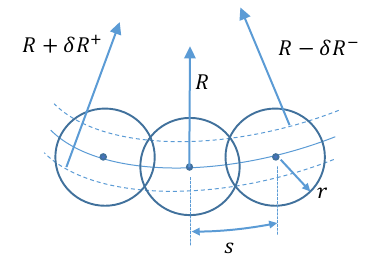
\includegraphics[scale=0.75]{Figures/mission_phase1_a}
\caption{Annular region contained within discrete circles}
\label{fig_mission_phase1_a}
\end{figure}

This suggests that the desired trajectory can be realized by a set of concentric circles whose radii $R_i$ are chosen to ensure that corresponding consecutive annular regions have non-zero overlap (see figure \ref{fig_mission_phase1_b}).

\begin{figure}
\centering
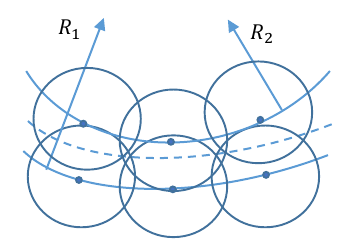
\includegraphics[scale=0.75]{Figures/mission_phase1_b}
\caption{Overlap between subsequent annular regions}
\label{fig_mission_phase1_b}
\end{figure}

The analytical values of $R_i$ can now be obtained recursively as follows:
\begin{enumerate}
\item Recurrence relation: $ R_k + \delta R_k^+ = R_{k-1} - \delta R_{k-1}^-$
\item Base case: $ R_1 + \delta R_1^+ = R_0 = 165$
\item Parametric dependence: $s=v \; t_s$
\end{enumerate}
where $v$ is the cruise airspeed and $t_s$ is the snapshot time gap. 
 
Clearly, the trajectory is completely specified once the functional relationships of $\delta R^+$ and $\delta R^-$ have been established. An instance of the passive trajectory for phase-1 is shown in figure \ref{fig_mission_phase1_c}.

\begin{figure}
\centering
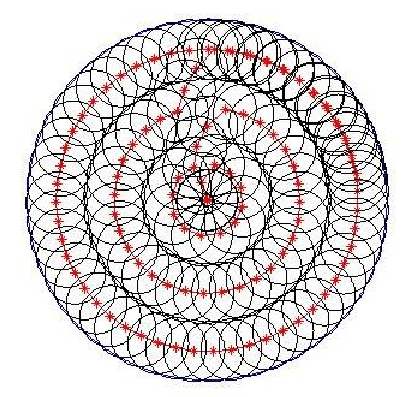
\includegraphics[scale=0.75]{Figures/mission_phase1_c}
\caption{Typical trajectory used for phase-1}
\label{fig_mission_phase1_c}
\end{figure}


\subsection{Phase-2: An active path to refine the estimates of sighted targets}

At the end of phase-1, each of the four targets $\xi^j$ is known to lie within a simply connected and provably convex region $\omega^j$ with probability 1. Define a suitable norm on the region $\| \omega^j\|$. For our purpose, the geometric area or the maximum distance between any two points on the periphery of the region are appropriate measures. We are interested in finding a trajectory $x^j_n$ for $n=1,2,3, \cdot , n_f$ such that the target region shrinks to a specified tolerance, i.e. the sequence $\omega_n^j$ converges so that $\| \omega^j_{n_f} \| < \| \omega_\gamma \|$  for a given tolerance $\| \omega_\gamma \|$. For an active trajectory, $x^j_n$ depends on $x^j_1, x^j_2, \cdot, x^j_{n-1}$.  Given this requirement, we can identify certain key characteristics of the trajectory:

\begin{itemize}
\item The trajectory must lead to convergence for any admissible $\xi^j$ and $\omega^j$
\item The discrete waypoints on the trajectory must be navigate-able within performance constraints
\item The determination of the trajectory must not be computationally intensive
\end{itemize}

For this phase of the mission, we augment the estimation procedure (see section \ref{sec:TPEA}) by keeping track of unsuccessful snapshots (those that did not contain the target) as well. The target region is then obtained by first evaluating the intersection of all successful snapshots and then exsecting the union of unsuccessful snapshots. The subsequent procedure is the same as before. Note that the estimation strategy guarantees that $\| \omega_n^j \|$ is a non-increasing sequence.

One possible active trajectory that satisfies the essential requirement of convergence can be obtained through heuristic arguments. Let $v$ be the cruise airspeed dictated by design for maximum endurance, $R_f$ be the radius of the field of view at the highest admissible altitude, $t_s$ be the snapshot gap time, and radius $R$ be an intrinsic parameter. Then:

\begin{enumerate}
\item Evaluate $y_n$ the centroid of $\omega_n$
\item Let $x_{n_1} = y_{n_1} + R \cos (v\;t_s/R), x_{n_2} = y_{n_2} + R \sin (v\;t_s/R)$ i.e. follow a circular path of radius $R$ centered at the centroid of the target region
\item Evaluate the field of view and check for presence of target. 
  \begin{enumerate}
  \item[a] If a target is found, evaluate $\omega_{n+1}$ using all the snapshots. Then repeat steps 1-3
  \item[b] Otherwise, set $\omega_{n+1} = \omega_{n}$  and repeat steps 2-3
  \end{enumerate}
\end{enumerate}

The exit criterion used for determining convergence has been taken to be $\| \omega_{n_f} \| < 1$ which approximately corresponds to the norm of the region being smaller than $\gamma = 1m$. The parameter $R$ is taken to be equal to $R_f \sim 30m$, and $v$ is taken to be $5 m/s$.

In words, this active path is composed of \lq shifting circles\rq where the changing circles correspond to levels of the algorithm. Several very interesting geometrical convergence statements can be proven. However, instead of delving deep into theoretical results, we briefly comment on the salient features of the process that are directly related to the key characteristics outlined above. 

\begin{itemize}
\item The algorithm is guaranteed to converge for any admissible target location and target region provided that $v<(2\pi R)/3$. In fact, the convergence is proportional to $\sqrt{n_l}$ where $n_l$ is the level of the algorithm. This follows from the fact that during each level of the algorithm the area of the region decreases on average by at least a factor of $1/3$ due to the following geometric result: A circle of radius $R$ can be equi- partitioned by $3$ circles of radii $R$ centered at the vertices of an equilateral triangle inscribed within the original circle.

\item The radii of the circles for any level of the algorithm is fixed to be $R = R_f \simeq 30m$. Since $v$ is taken to be $5 m/s$, the required rate of turn of very low and the waypoints can be navigated easily.

\item The simplicity and strength of this method lies in the recursion among levels. The definition of the trajectory is dependent on the target region only through the centroid. Thus, no special treatment is required as the target region shrinks. The altitude is kept fixed at the highest admissible value. Clearly, the generation of waypoints is computationally simple.

\item The performance of the algorithm is fairly robust with respect to small variations in the possible parameter set - $R,v, $ altitude etc. 

\end{itemize}

An instance of the refinement procedure for a randomly generated target starting from a single snapshot (worst case scenario at the end of phase-1) is shown in figure \ref{fig_mission_phase2_a}. The \lq x\rq mark is the true target, the \lq + \rq marks are estimates returned by the camera, the diamonds are processed target locations, and \lq * \rq denote the target region. A portrait of the successful and unsuccessful snapshots is shown in figure \ref{fig_mission_phase2_b}. Figure \ref{fig_mission_phase2_c} plots the convergence history of the algorithm through a geometrical as well as an exact measure.

\begin{figure}
\centering
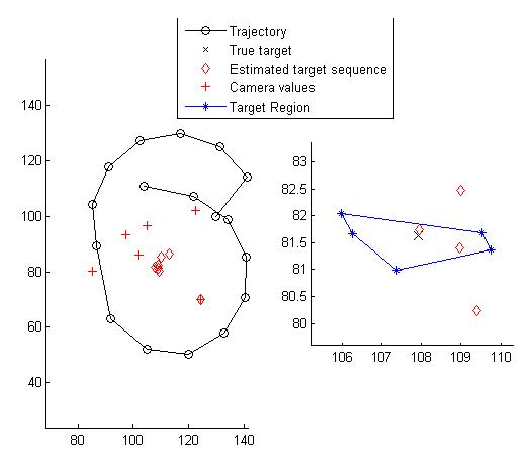
\includegraphics[scale=0.75]{Figures/mission_phase2_a}
\caption{An instance of the refinement procedure}
\label{fig_mission_phase2_a}
\end{figure}

\begin{figure}
\centering
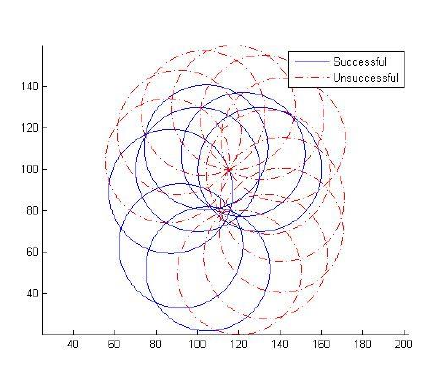
\includegraphics[scale=0.75]{Figures/mission_phase2_b}
\caption{A portrait of the successful and unsuccessful snapshots}
\label{fig_mission_phase2_b}
\end{figure}

\begin{figure}
\centering
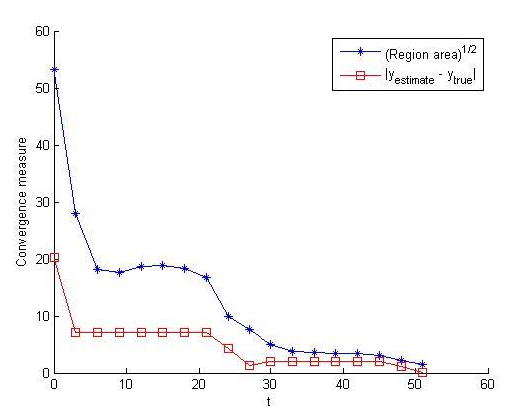
\includegraphics[scale=0.75]{Figures/mission_phase2_c}
\caption{Convergence history of the algorithm}
\label{fig_mission_phase2_c}
\end{figure}


\subsection{Target position estimation scheme}
\label{sec:TPEA}

Skynet's target position estimation algorithm is based upon the following two observations:

\begin{enumerate}
\item The camera reports an estimate only when the true target is located within the FOV. Hence, after $K_j$ successful snapshots for the $j^{th}$ target, the target must be located in $\cap_i^{K_j} F_{j_k}$ with probability $1$.

\item The estimates $y_{est_{j_k}}$ returned from the camera for the $j^{th}$ target are drawn from a bivariate normal distribution with mean $(y_{true_{j_1}}, y_{true_{j_2}})$ and finite expectation. The maximum likelihood estimator for this case is exactly the sample mean 

\[ (\hat{y}_{j_1}, \hat{y}_{j_2}) = \frac{1}{K_j} \left( \sum\limits_1^{K_j} y_{est_{j_{k_1}}}, \sum\limits_1^{K_j} y_{est_{j_{k_2}}} \right)\]

\end{enumerate}

The following asymptotic results provide theoretical reliability to the two measures mentioned above

\begin{enumerate}
\item Let $F_i=\{y : \| (y_1,y_2) -(y_{i_1},y_{i_2})\| \leq r, \| (\xi_1,\xi_2) -(y_{i_1},y_{i_2})\| \leq r \}$ denote circular areas with radius $r$ centered at $y_i$ that all necessarily contain the point $\xi$. Further let $y_i$ be drawn from a uniform random distribution in $\mathbb{R}^2$. Then, $P(\| y_n - \xi \| > \delta) \rightarrow 0 \; \; \forall \; \; y_n \in \cap_i^n F_i, \; \delta>0 $ as $n \rightarrow \infty$. 

In other words, the intersection of the random circles converges to the common point. Hence, if we take enough snapshots, the fields of view alone would be enough to provide us with the true location of the targets.

\item The maximum likelihood estimator is asymptotically convergent (i.e. consistent)

Hence, if take enough snapshots, the random estimates from camera alone would provide us with the true location of the targets.
\end{enumerate}

The actual implementation of the above procedure is relatively complicated. While the sample mean of estimates is easy to calculate, the intersection of circles is more involved. Similarly, the process of ensuring that the final estimate falls within this intersection is another task. Skipping over the details for brevity, we provide here a flowchart of the process for each target:

\begin{enumerate}
\item 
1. Find a discrete representation of the region of intersection of the FOV circles - $I$

Scheme:
The intersection of $n$ circles (that all contain a common point) results in $\left( \begin{array}{c} n  \\ 2 \end{array} \right)$ intersection points. Out of these, only $p \leq n$ points lie on the periphery of the intersection of the circles. The necessary and sufficient condition for these points $z_m$ for $m = 1,2, \cdot , p$ is given by
\[ \|z_m - y_i\| \leq R_i \textrm{ for } i=1,2,\cdot,n  \]

where $y_i$ are circle centers, and $R_i$ the radii.

Owing to the convexity of circular arcs, these $p$ points 
result in a $p$-sided convex polygon (see figure \ref{fig_mission_tpea_a}).

\begin{figure}
\centering
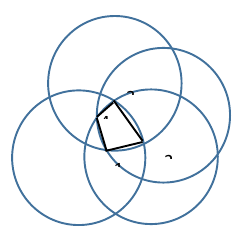
\includegraphics[scale=1]{Figures/mission_tpea_a}
\caption{Region that contains the target with probability 1}
\label{fig_mission_tpea_a}
\end{figure}

\item  Find the sample mean of the estimates returned by the camera $\hat{y}$

\item  Check if $\hat{y} \in I$. If yes, report $\hat{y}$ as the final estimate (see figure \ref{fig_mission_tpea_b}).

Scheme:
Standard geometric algorithm for detecting if a point lies
inside a convex polygon. 

\begin{figure}
\centering
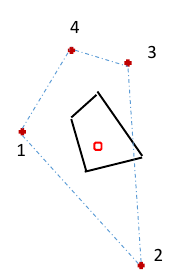
\includegraphics[scale=0.75]{Figures/mission_tpea_b}
\caption{MLE within geometric requirements}
\label{fig_mission_tpea_b}
\end{figure}


\item  If $\hat{y} \not\in I$ report $y_{target}$ as the point in $I$ that is \lq close\rq to $\hat{y}$.

Scheme:
Find the point of intersection of the line joining centroid 
of the polygon and $\hat{y}$  with the perimeter of the polygon. (see figure \ref{fig_mission_tpea_c})

\begin{figure}
\centering
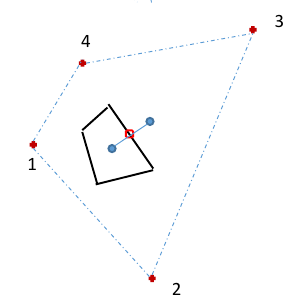
\includegraphics[scale=0.75]{Figures/mission_tpea_c}
\caption{Geometric correction to MLE}
\label{fig_mission_tpea_c}
\end{figure}


\end{enumerate}

Figure \ref{fig_mission_tpea_d} shows the advantage of this estimation method during actual simulations. The \lq x\rq marks are the true targets, the \lq +\rq marks are estimates returned by the camera, and the squares are processed target locations.

\begin{figure}
\centering
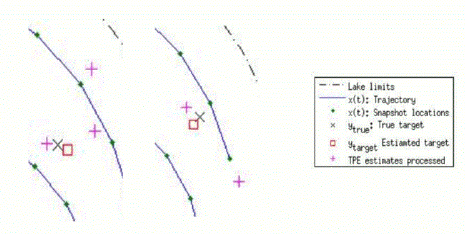
\includegraphics[scale=0.75]{Figures/mission_tpea_d}
\caption{Performance of estimation algorithm}
\label{fig_mission_tpea_d}
\end{figure}

\subsection{Statistical measure of score and mission time}

As per the analysis of the aircraft performance group, the finalized aircraft design was expected to have maximum endurance near stall speed. For this purpose, the airspeed for Phase-2 was simulated at $5m/s$. (Actual flight tests later revealed that the airplane stalled around $7m/s$ and, incidentally, could operate stably only above $9m/s$). 

Similarly, the optimal rate of climb at the beginning of Phase-1 was simulated as per design values. The only free parameter remaining was the cruise speed during phase-1. Towards this aim, a parametric study with cruise airspeed was conducted by gathering statistics over 100 realizations of the target locations.

\begin{figure}
\centering
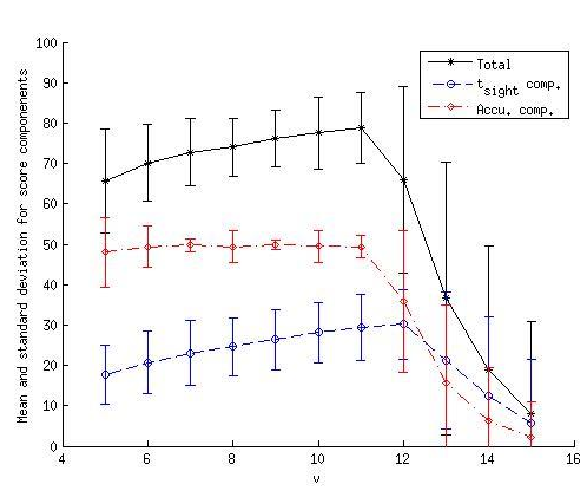
\includegraphics[scale=0.75]{Figures/mission_stats_a}
\caption{Mean and standard deviation for score components}
\label{fig_mission_stats_a}
\end{figure}

Figure \ref{fig_mission_stats_a} plots the variation of the sample mean of the two components of score ($\beta/t_{sight}$ and $\alpha/ \sum_{i=1}^4 \max(\gamma, \|y_{target} - y_{true} \|)$) and the total score along with their standard deviations as error bars. We note that

\begin{itemize}
\item The accuracy component is very close to its maximum value ($\sim 50$) for $v\leq 11m/s$
\item The $t_{sight}$ component increases with $v$ for $v \leq 12 m/s$ after which the battery gets consumed for some realizations even before phase-1 can be completed
\item The accuracy component for $v=12 m/s$ is reduced due to excessive battery consumption during phase-1
\item From a-c, we conclude that $v = 11m/s$ is the ideal cruise speed for phase-1
\end{itemize}

It is important to mention that these observations should have been ideally dictated by actual flight tests rather than empirical estimates. However, the final implementation, integration and debugging of the airplane system did not leave much time for testing and fine tuning.

\begin{figure}
\centering
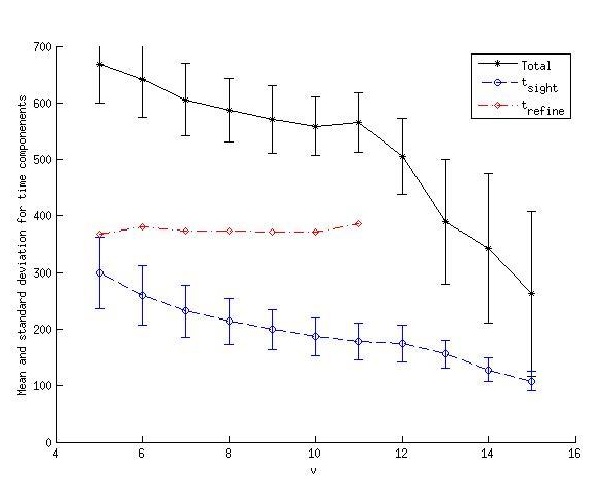
\includegraphics[scale=0.75]{Figures/mission_stats_b}
\caption{Mean and standard deviation for time components}
\label{fig_mission_stats_b}
\end{figure}

Figure \ref{fig_mission_stats_b} plots various components of mission time for such cases where all targets could be located before the battery was consumed. As expected, $t_{sight}$ does decrease with $v$ under this restriction. The refinement times start to go down for $v \geq 12 m/s$ as the targets are not fully refined before the battery is consumed, and are therefore not plotted on the graph below.

Finally, the statistics for the chosen parameter values are tabulated below. This is the theoretical expectation of the mission values.

\begin{center}
    \begin{tabular}{ | c | c | c | c | }
    \hline
    Quantity & Component & Mean & Standard dev. \\
    \hline
    Score & Total & 78.3 & 9.3 \\
    		  & Accuracy & 49.3 & 4.1 \\
     	  & $t_{sight}$ & 29.0 & 8.2 \\ \hline
    Time  & Total & 557.0 s & 56.1 s \\
     	  & $t_{sight}$ & 180.9 s & 33.0 s \\ \hline
    \end{tabular}
\end{center}

		\label{Mission}

		\section{Airframe Design}
			\label{Vehicle}

			\subsection{Propulsion System Analysis}

			The propulsion system analysis was performed in three parts:
			\begin{enumerate}
				\item Propeller analysis
				\item Motor analysis
				\item Propeller and Motor matching
			\end{enumerate}

			\subsubsection{Propeller Analysis}

			For the propeller analysis, we used wind tunnel experimental data from the UIUC Propeller Data Site \footnote{http://aerospace.illinois.edu/m-selig/props/propDB.html}. The exact same propeller data was unavailable in the database, so we used a very similar propeller (Graupner CAM Slim 9x5) albeit from a different manufacturer.

			The data was given in terms of the rotations per second instead of the angular velocity and hence, the following scaling had to be performed

			\begin{eqnarray*}
				\lambda &=& \frac{J}{\pi} \\
				C_T &=& \left( \frac{2}{3} \right)^3 C_T ^ \prime \\
				C_P &=& \frac{1}{\pi} \left( \frac{2}{3} \right)^3 C_P ^ \prime \\
				\eta &=& \eta ^ \prime
			\end{eqnarray*}
			where $\lambda$ is the advance ratio based on the angular velocity, $J$ is the advance ratio based on the rotations per second, $C_T$ is the thrust coefficient, $C_P$ is the power coefficient and $\eta$ is the propeller efficiency. The primed quantities are the ones reported in the database.

			\subsubsection{Motor Analysis}
			The motor analysis was performed by using the standard electric motor model. The motor speed constant, motor resistance and the no-load motor current were obtained from experimentally measured values on the manufacturer's website \footnote{http://www.maxxprod.com/pdf/HC2808-xxxx.pdf}.

			The values of the model constants are reported below:
			\begin{eqnarray*}
				K_v &=& 980 \left( \frac{2 \pi}{60} \right) \; rad/s/volt \\
				R_m &=& 0.220 \; \Omega \\
				i_0 &=& 0.4 \; A
			\end{eqnarray*}

			\subsubsection{Propeller and Motor Matching}
			For a given free-stream velocity, the required torque for the propeller was calculated as a function of the angular velocity of the propeller. For the motor, the torque generated was calculated as a function of the angular velocity. By matching these two torques, we solved for the angular velocity and obtained the total propulsive efficiency. This process is illustrated in Figure~\ref{fig:prop-motor1}.
			\begin{figure}[h!]
				\centering
				\begin{subfigure}[b]{0.49\textwidth}
					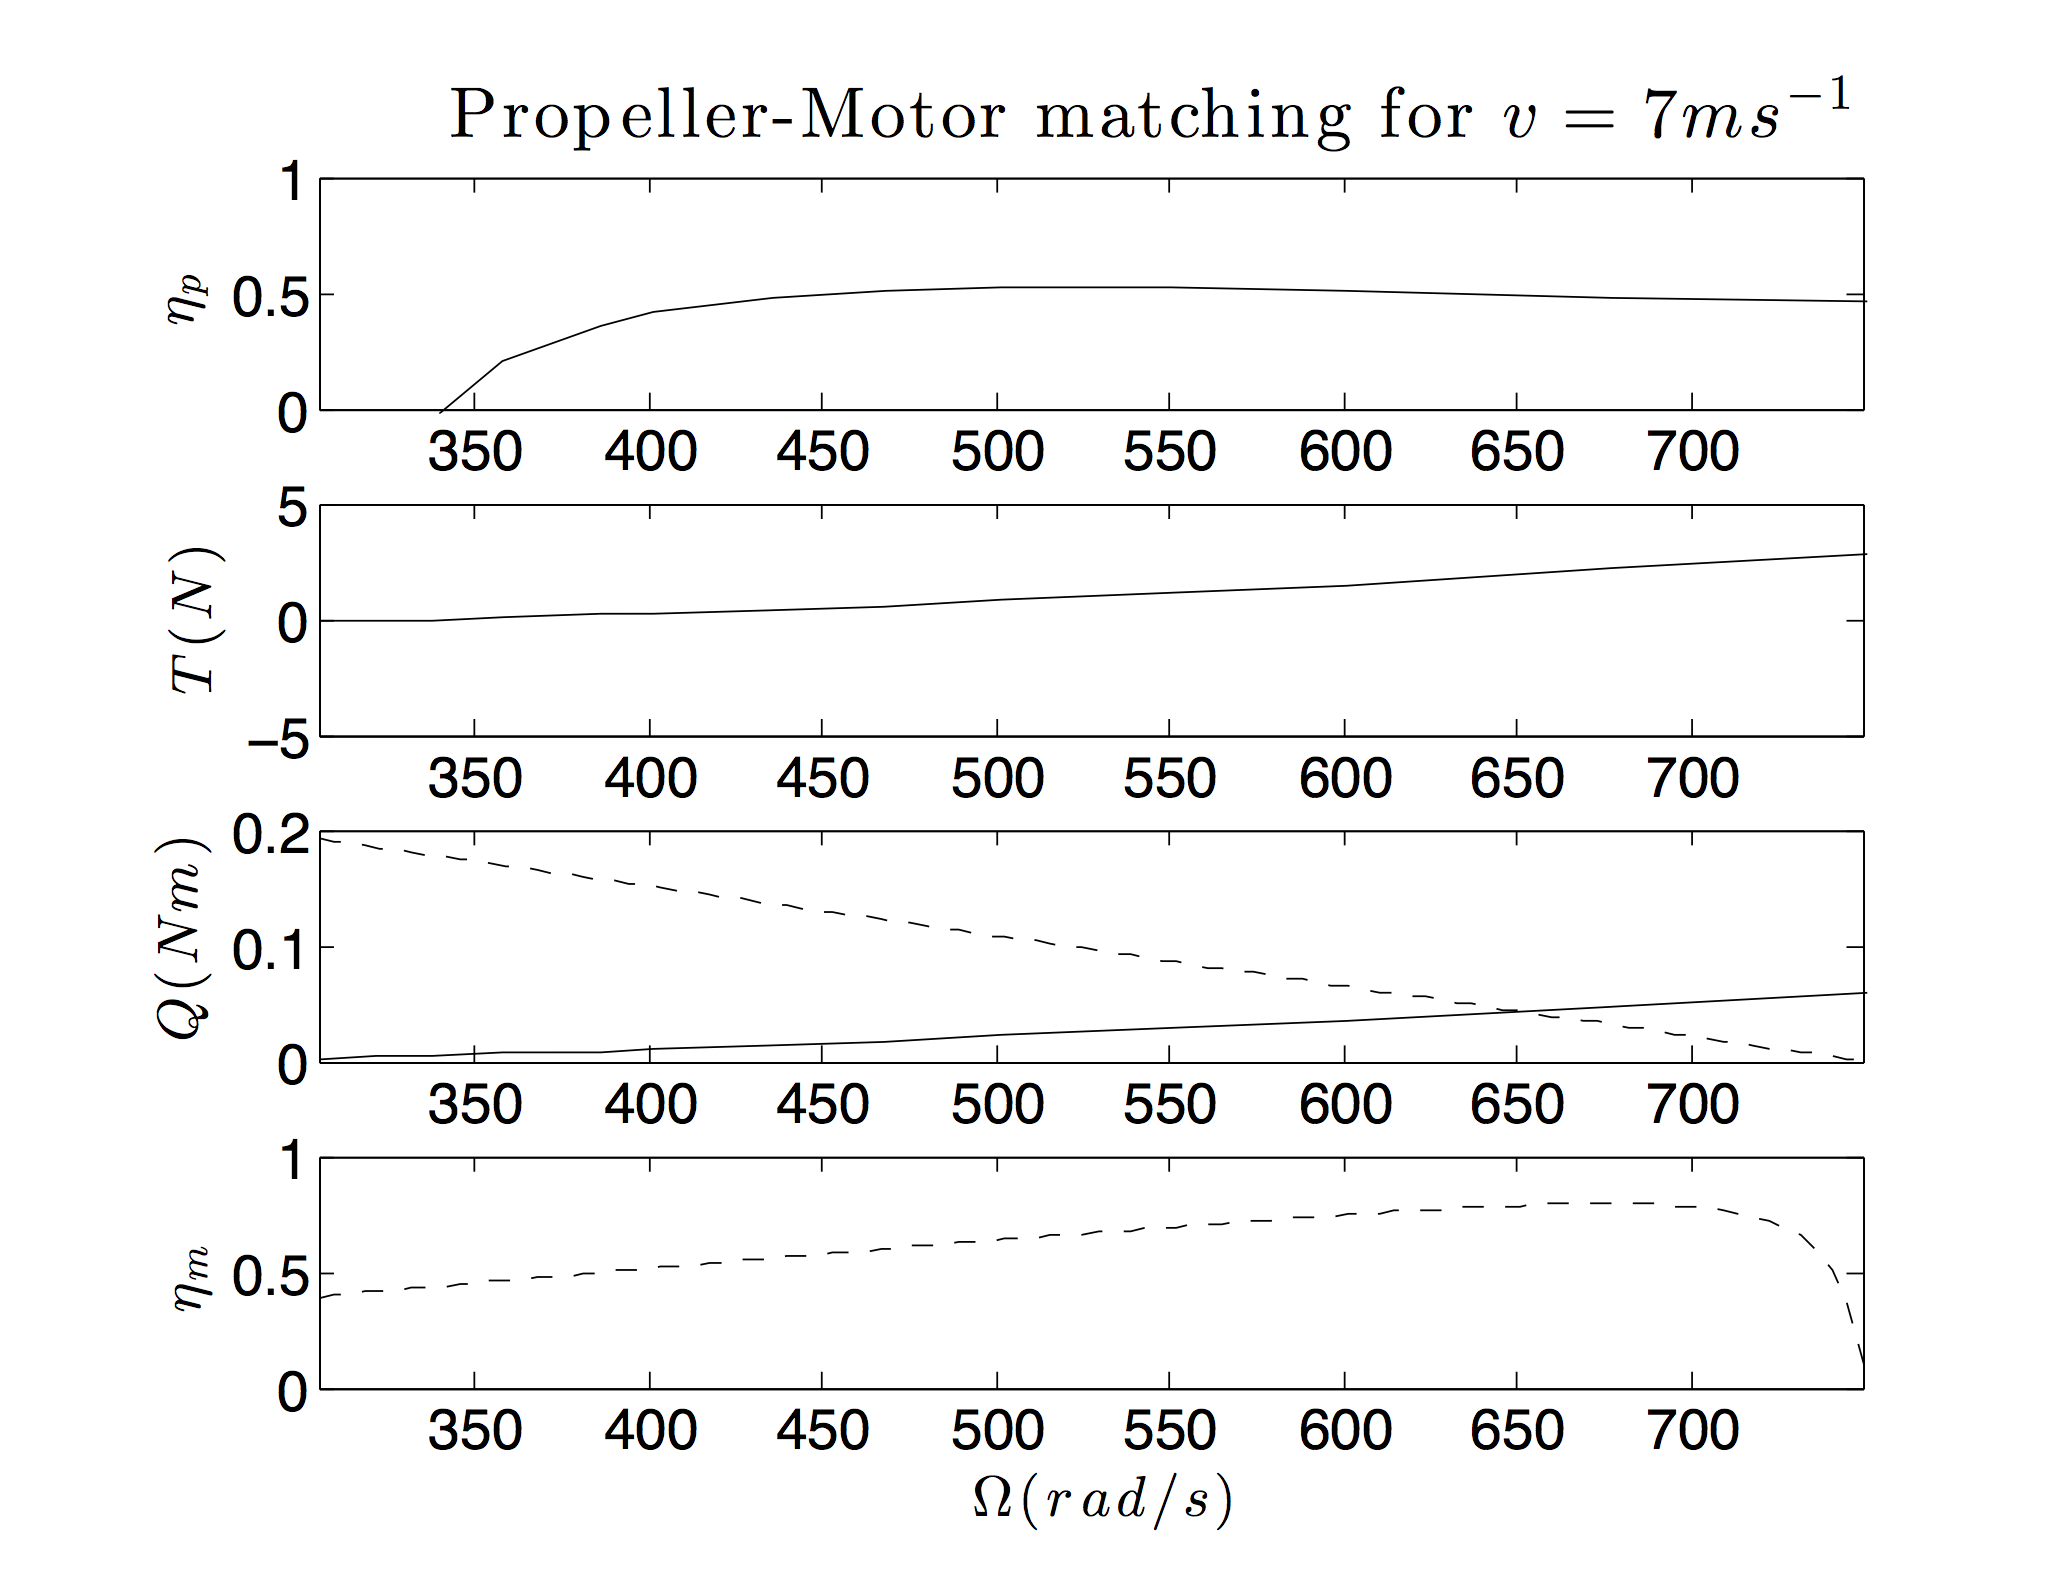
\includegraphics[width=\textwidth]{Figures/PS3/propmotor_v07p0.png}
					\caption{$v = 7 \; m/s$}
				\end{subfigure}
				\begin{subfigure}[b]{0.49\textwidth}
					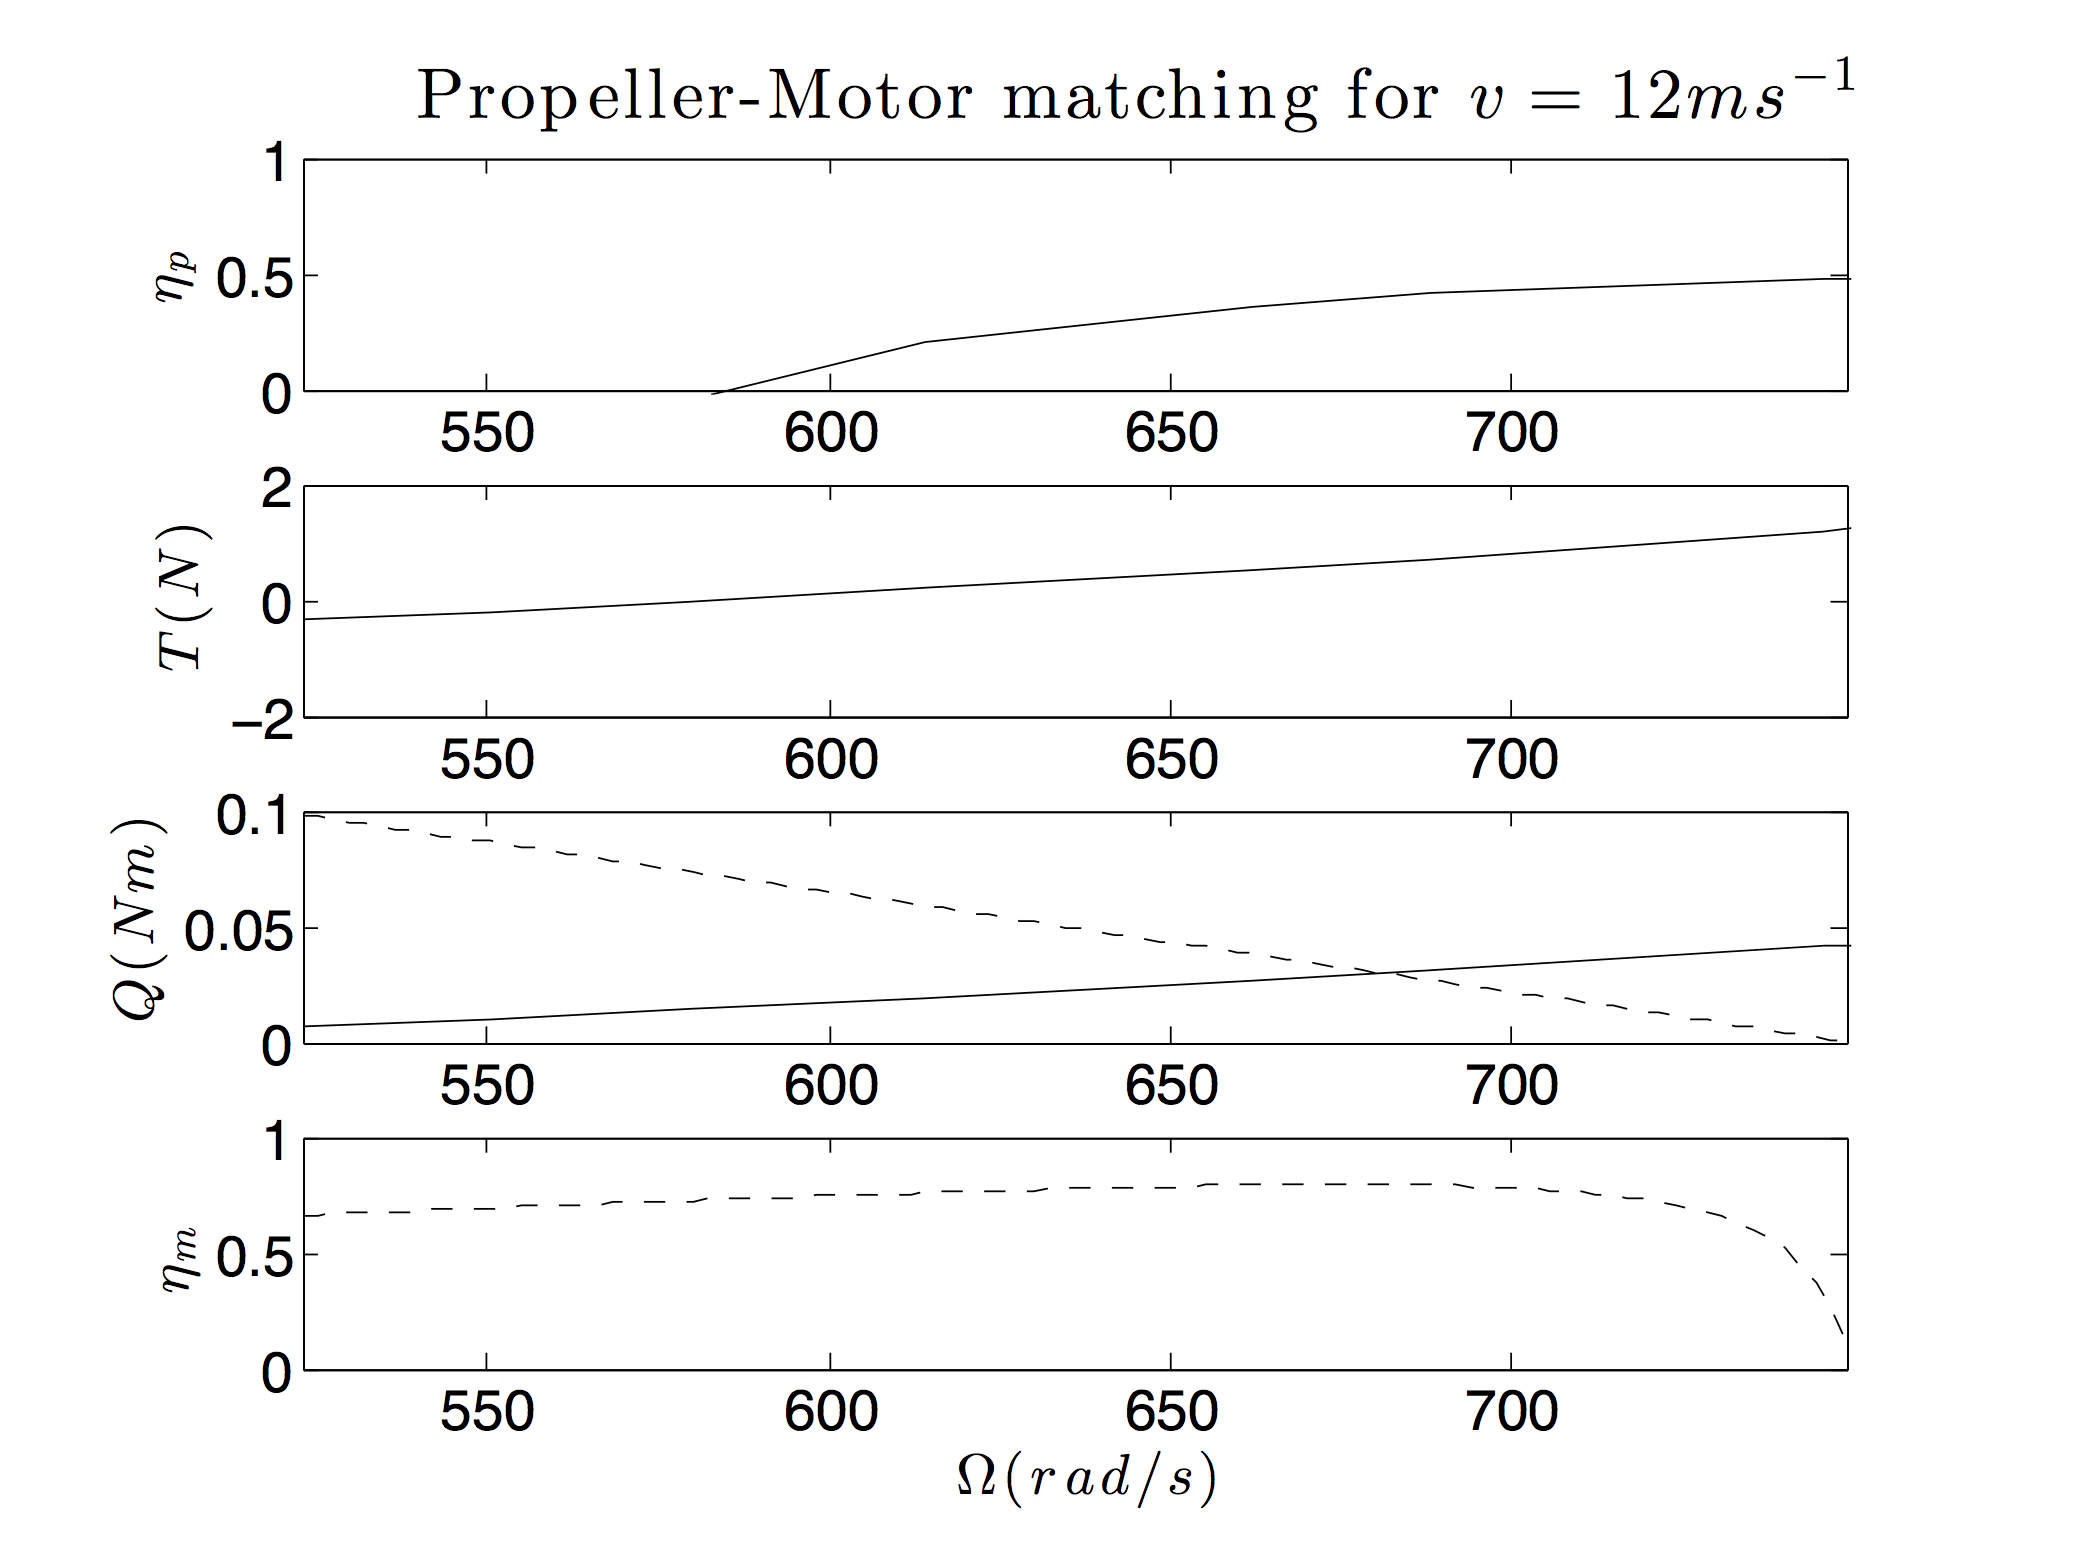
\includegraphics[width=\textwidth]{Figures/PS3/propmotor_v12p0.png}
					\caption{$v = 12 \; m/s$}
        \end{subfigure}%
        \caption{Propeller-Motor matching shown graphically. Solid lines: propeller curves. Dashed lines: Motor curves}\label{fig:prop-motor1}
    \end{figure}

    For the $7 \; ms^{-1}$ case, we see that the propeller efficiency, $\eta_p$ peaks at very low angular velocities and hence the total propulsive efficiency is poor. For the $12 \; ms^{-1}$ case, the propeller efficiency, $\eta_p$ peaks at high angular velocities which again leads to a low total propulsive efficiency. Optimizing the total propulsive efficiency over different airspeeds, we get the best motor-propeller matching illustrated in Figure~\ref{fig:prop-motor2}

    \begin{figure}[h!]
    	\centering
    	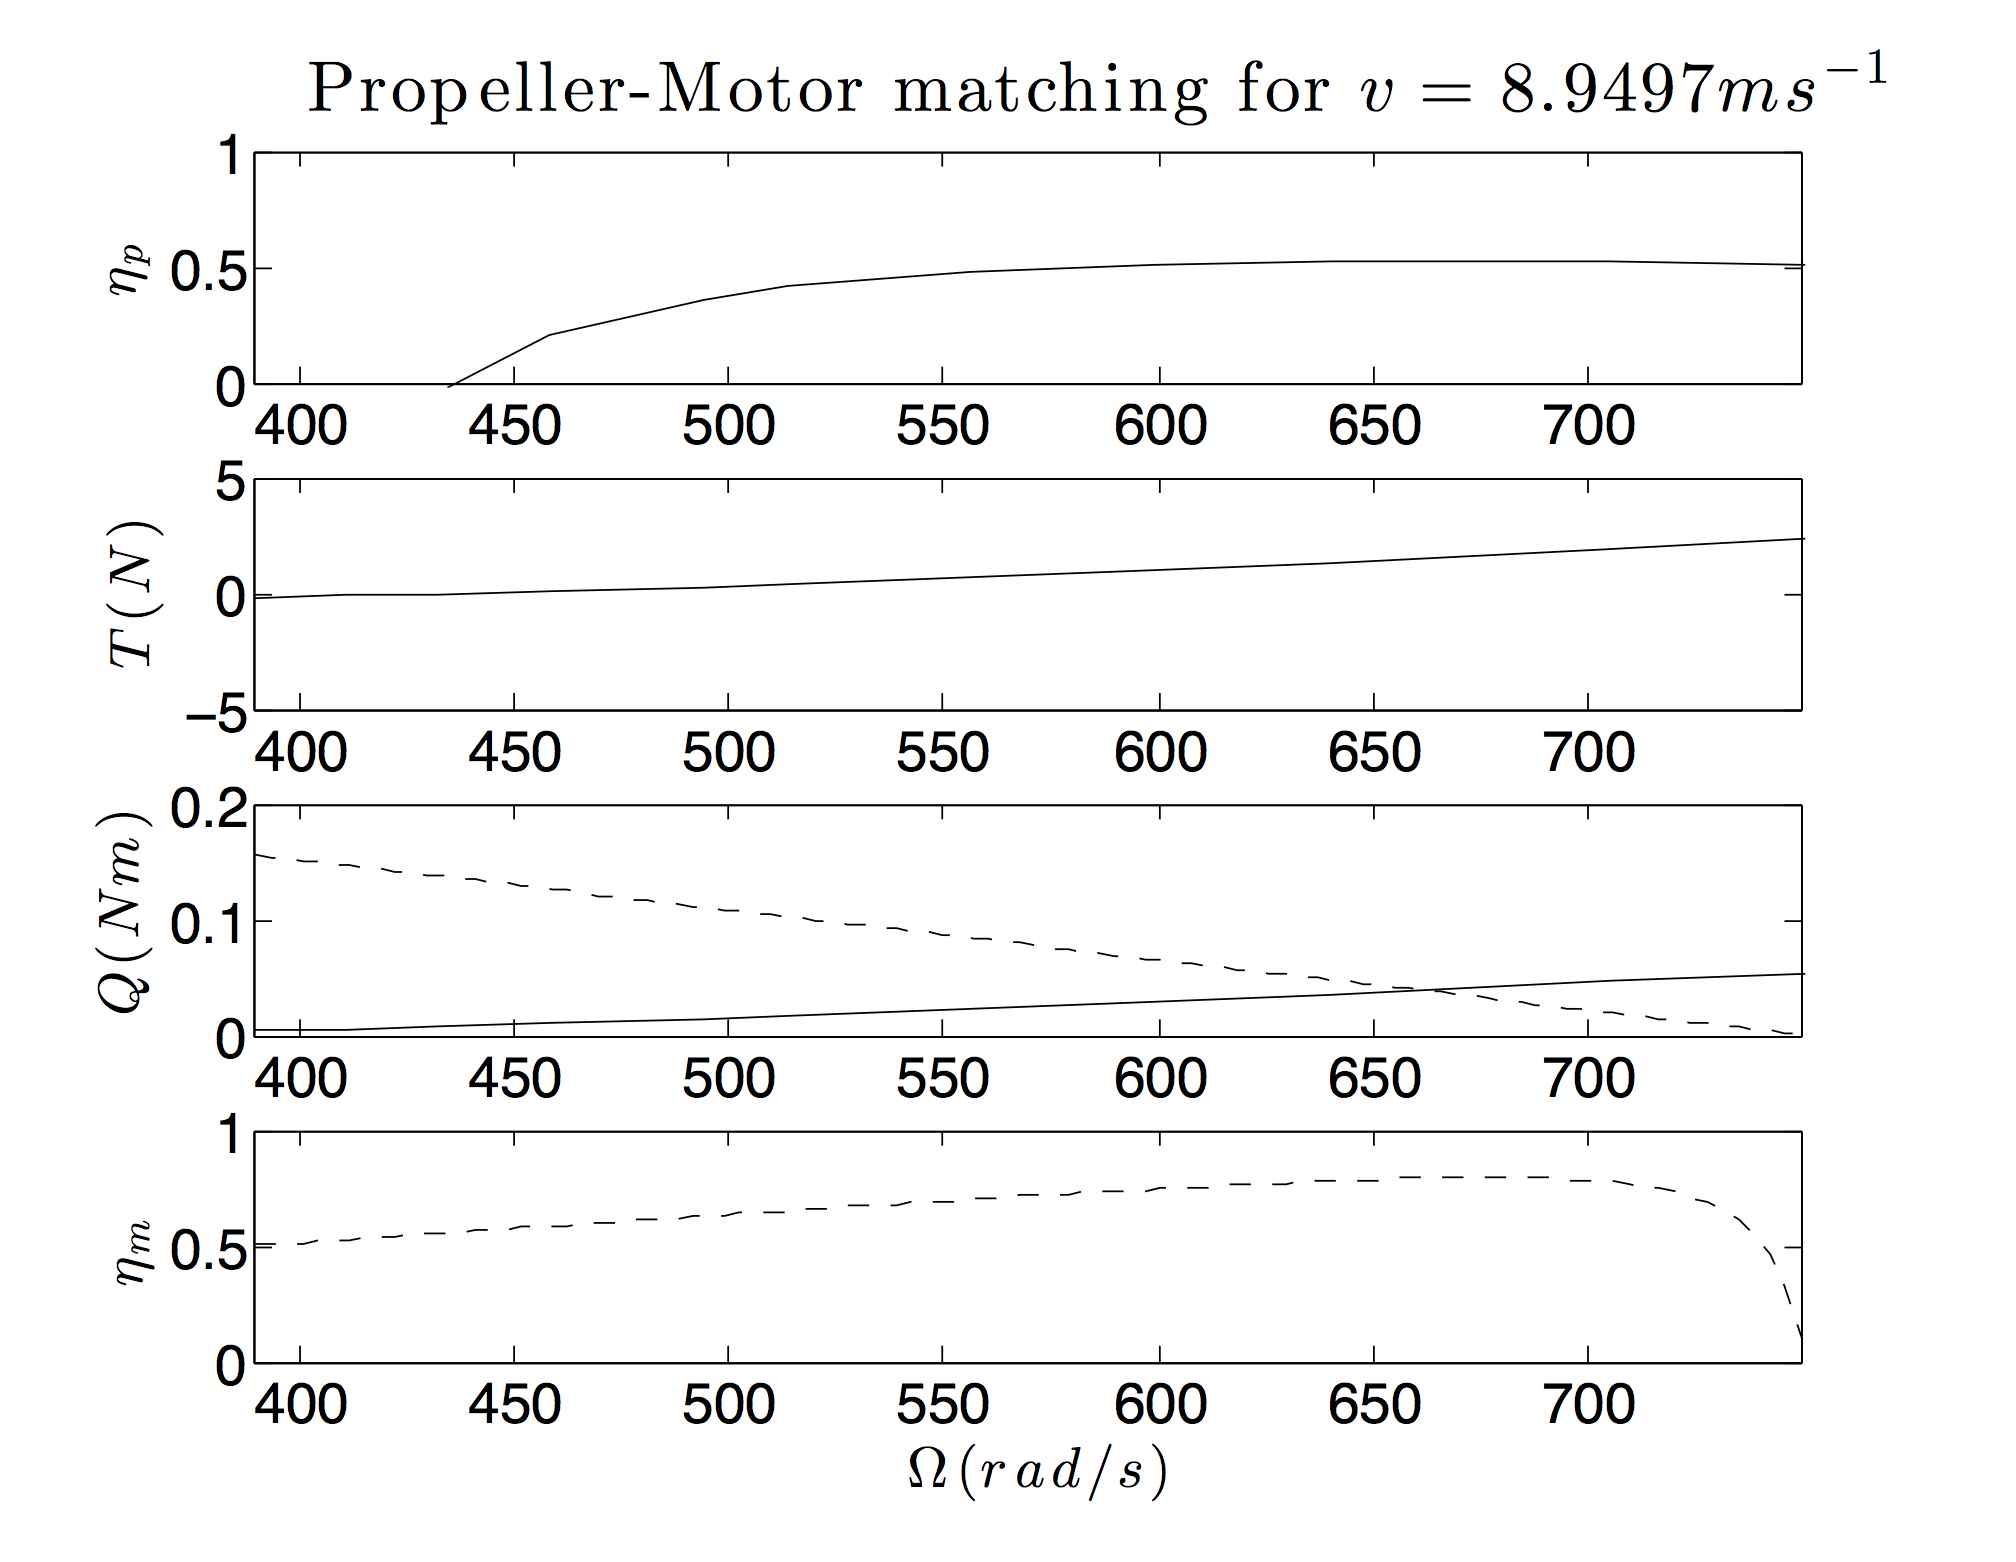
\includegraphics[width=\textwidth]{Figures/PS3/propmotor_opt.png}
    	\caption{Optimal Propeller-Motor matching shown graphically. Solid lines: propeller curves. Dashed lines: Motor curves}\label{fig:prop-motor2}
    \end{figure}

    The total propulsive efficiency and the thrust are plotted against airspeed in Figure~\ref{fig:teff-thrust}.

    \begin{figure}[h!]
    	\centering
    	\begin{subfigure}[b]{0.49\textwidth}
    		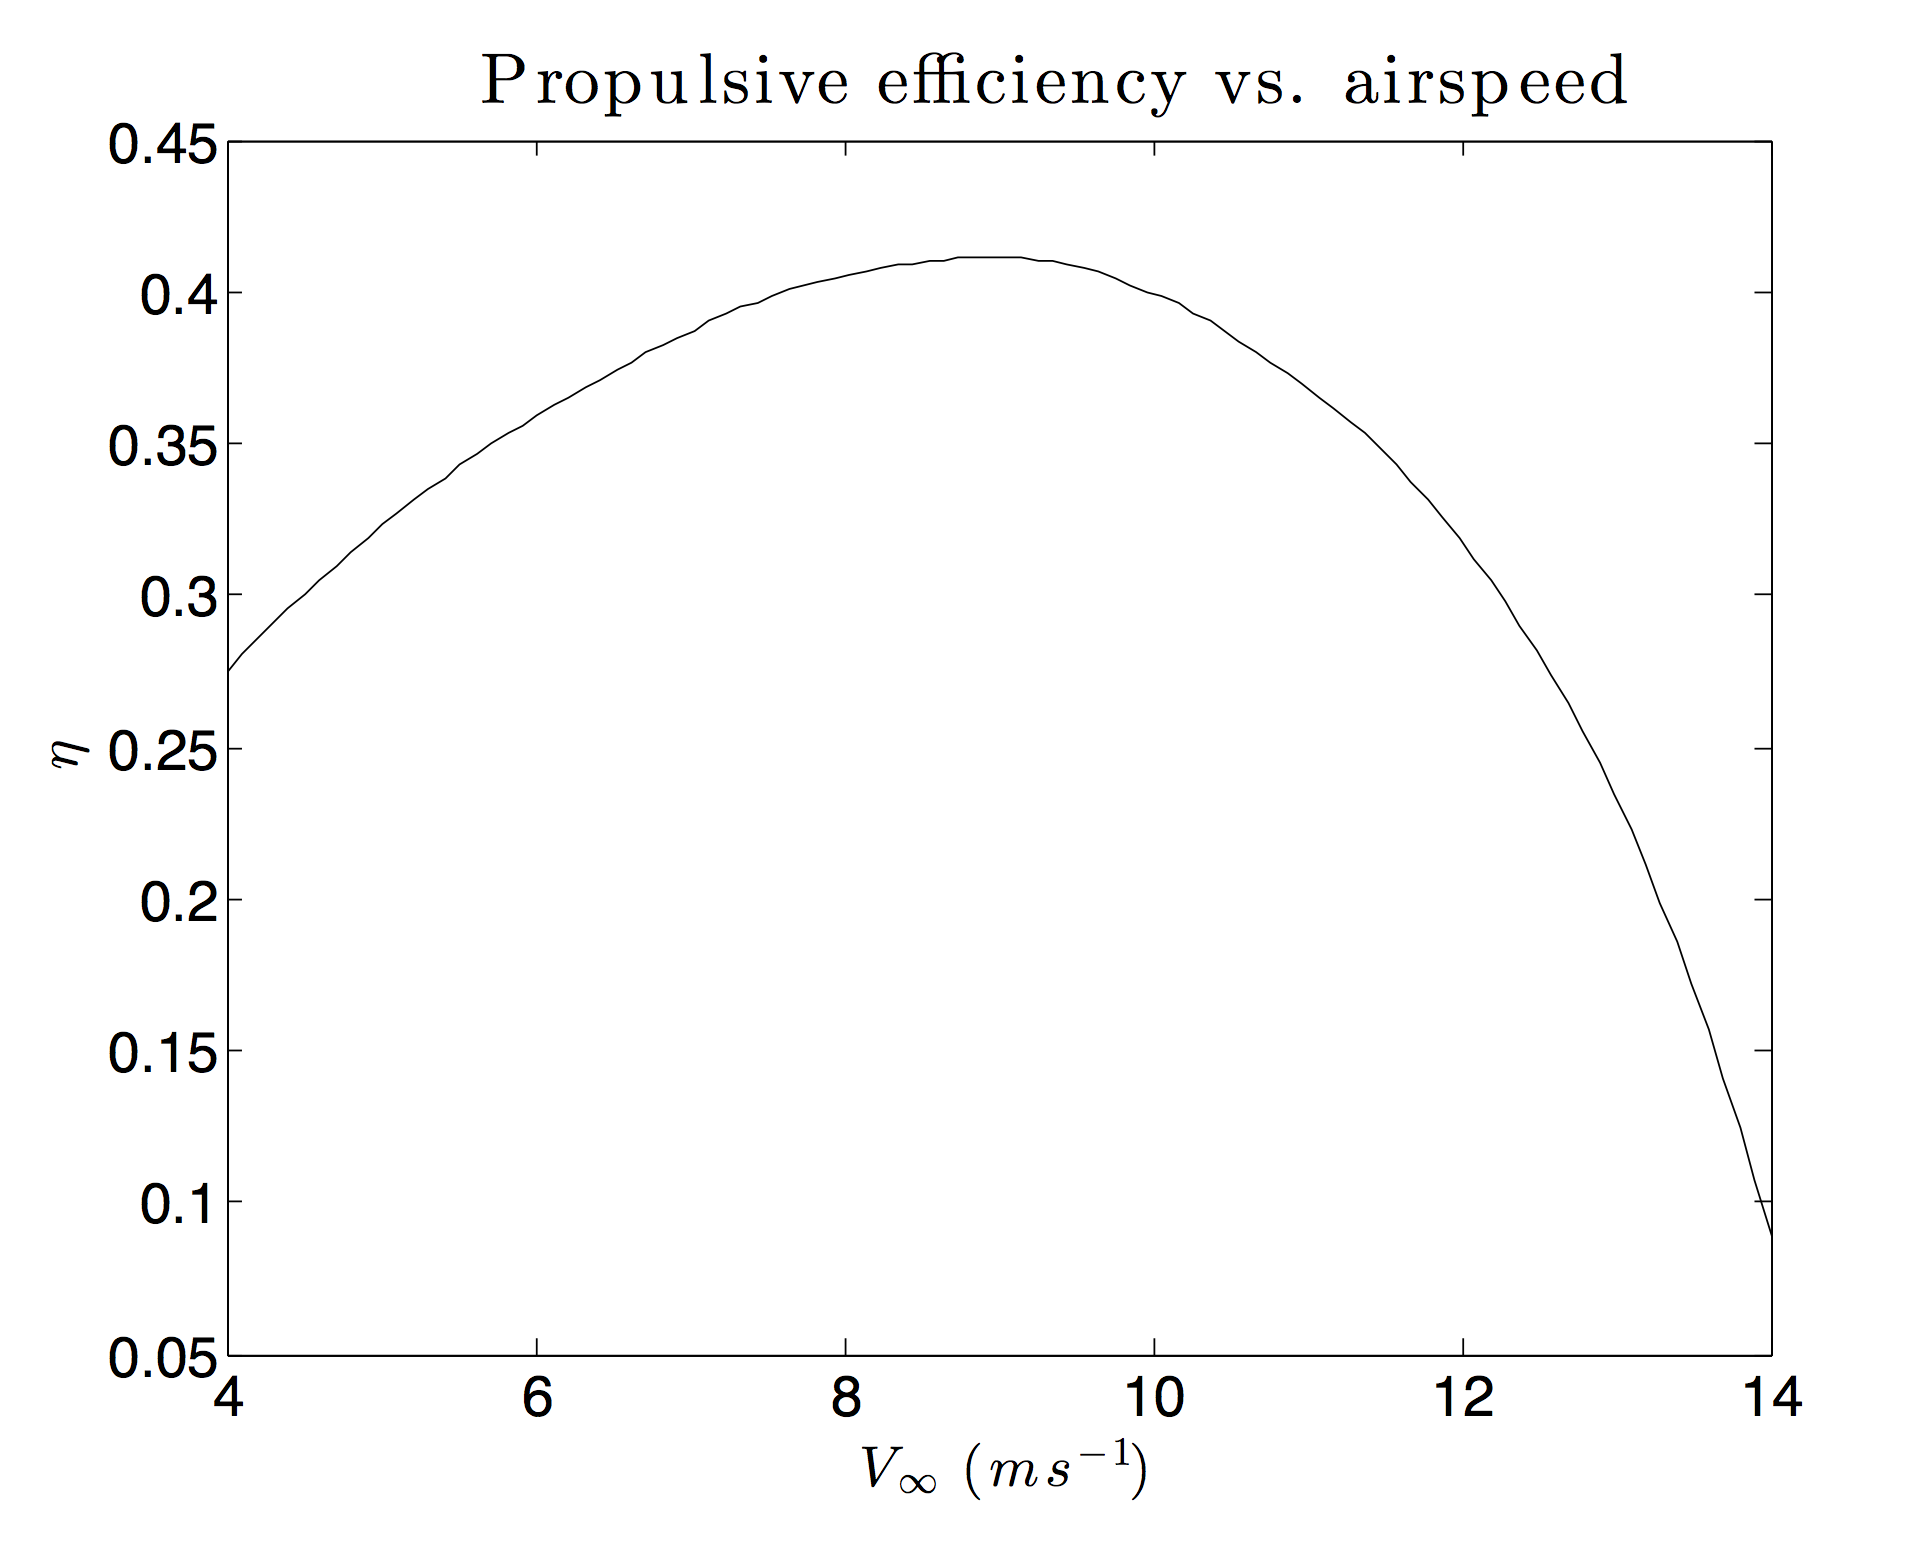
\includegraphics[width=\textwidth]{Figures/PS3/Teff.png}
    		\caption{Plot of the total propulsive efficiency against airspeed}
    	\end{subfigure}
    	\begin{subfigure}[b]{0.49\textwidth}
    		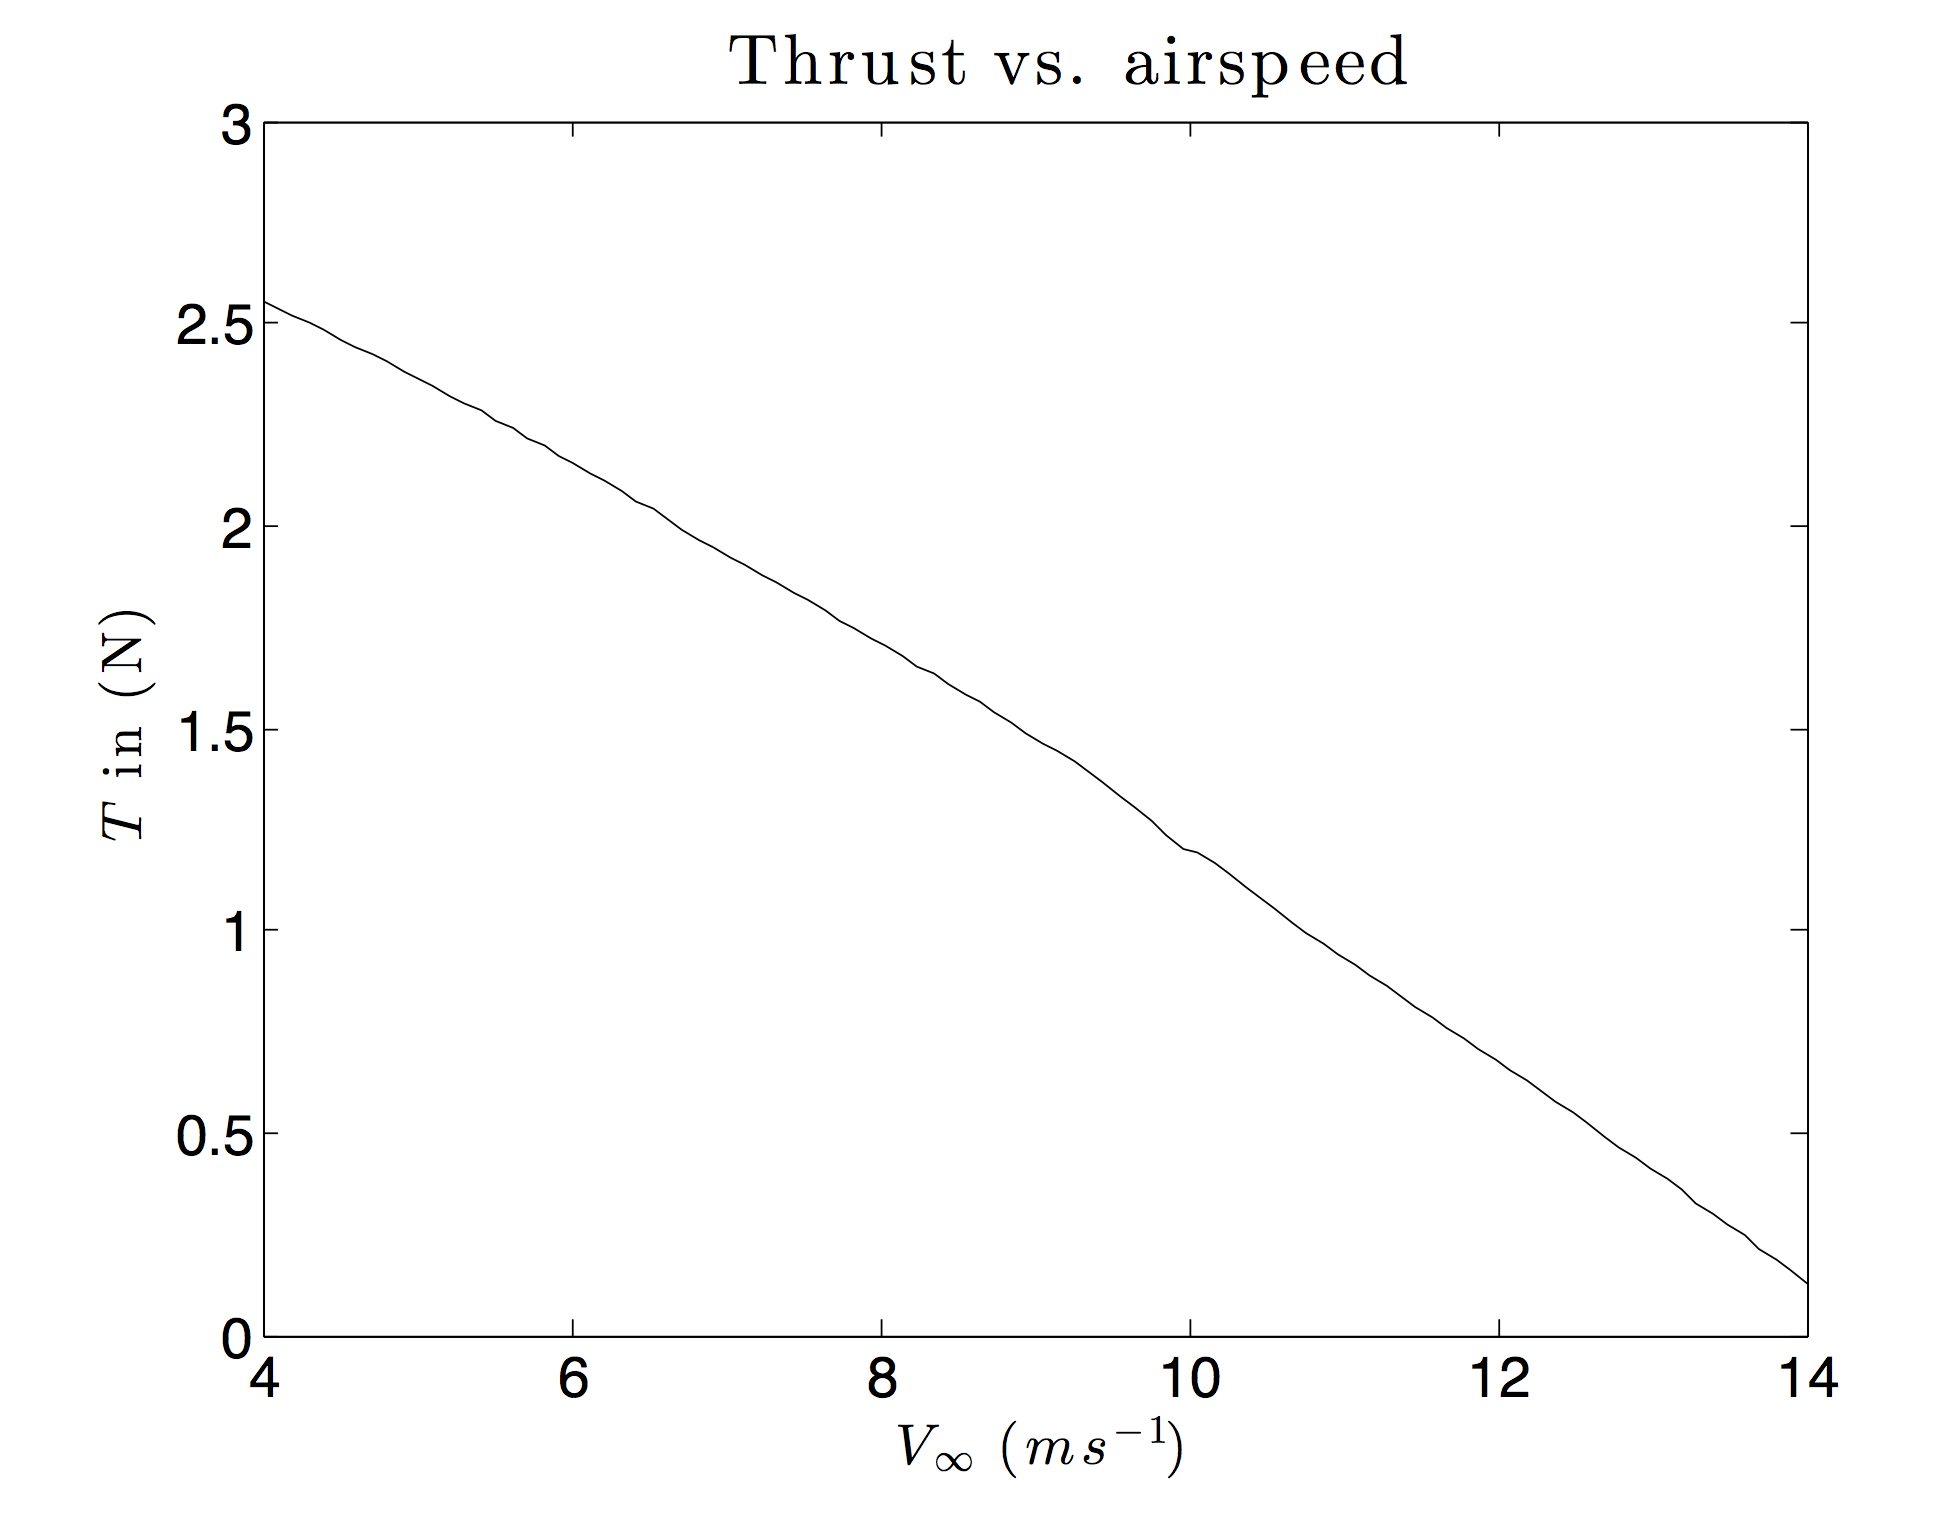
\includegraphics[width=\textwidth]{Figures/PS3/Thrust.png}
    		\caption{Plot of the total thrust against airspeed}
        \end{subfigure}%
        \caption{Thrust and efficiency plots}\label{fig:teff-thrust}
    \end{figure}

    \subsection{Design Approach}
    \label{DsignAppr}

    For our mission plan, it is critical that we climb to an altitude of $400 ft$ as fast as we can to efficiently scout the search area and sight all four targets as soon as we can. Hence, the rate of climb for our airplane is of crucial importance. In addition to this, the endurance of our aircraft is also very important since the allowed battery consumption is very limiting. We designed our aircraft mainly based on these two considerations.

    First, we obtained the drag polar for a generic 2D semi-symmetrical airfoil section (Clark-Y) in XFLR5 that we used as our first estimates for our full aircraft drag polar. From some preliminary weight estimates, we allotted a $450g$ weight budget for our aircraft. Using this weight and the 2D drag polars data, we found the wing area that would maximize our rate of climb using the data from the analysis of the propulsion system. We chose a taper ratio of $0.5$ for our wing. This choice was influenced by structural constraints on the total root bending moment and the stall characteristics so that in the event of a stalled aircraft, aileron control is not lost. Then, we assumed an aspect ratio of $6.8$ (that of the Bixler 2). This allowed us to construct a wing in XFLR5 to get a more realistic drag polar. This process was repeated iteratively until convergence. However, we changed our aspect ratio to $10$ since we felt it would be possible to make a wing with that aspect ratio that is still rigid enough.

    After this preliminary analysis, we did the same analysis with different airfoil sections and chose the SD-7037 airfoil section since the predicted $(L/D)_{max}$ was the highest for this airfoil. The effect of the choice of airfoil section on the climb performance was found to be minimal and hence we were able to perform a decoupled analysis for the choice of airfoil sections.

    Then, we calculated the horizontal stabilizer area from considerations of the longitudinal stability that were backed by Vortex Lattice Model predictions. The vertical stabilizer size was chosen based on previous aircraft designs similar to our aircraft and then validated using stability analysis in AVL.

    \begin{figure}[h!]
    	\centering
    	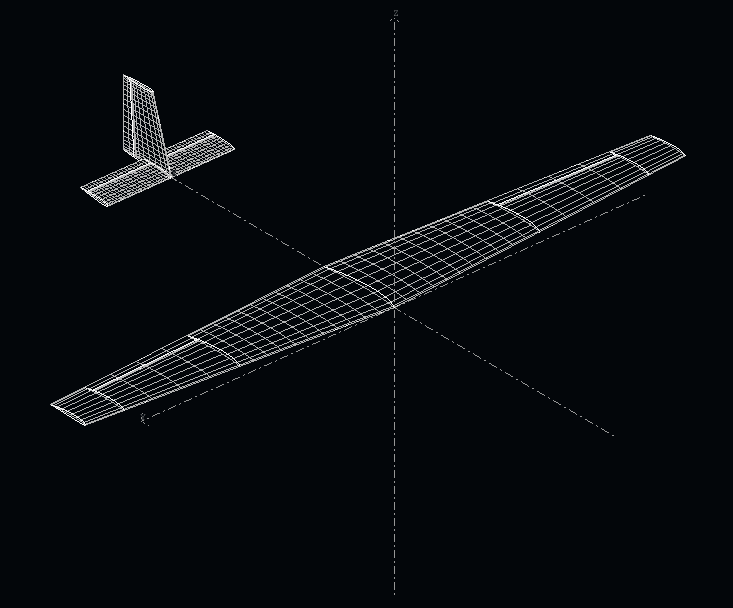
\includegraphics[width=0.7\textwidth]{Figures/PS3/SkynetV3_XFLR_pic.png}
    	\caption{VLM model of our design in XFLR5}\label{fig:vlm-design}
    \end{figure}

    \subsection{Performance Characteristics}
    \label{PerfChar}

    The different performance parameters of our design as predicted by XFLR5 are shown in Figures~\ref{fig:cl-alpha} to \ref{fig:power-cons}.

    \begin{figure}[h!]
    	\centering
    	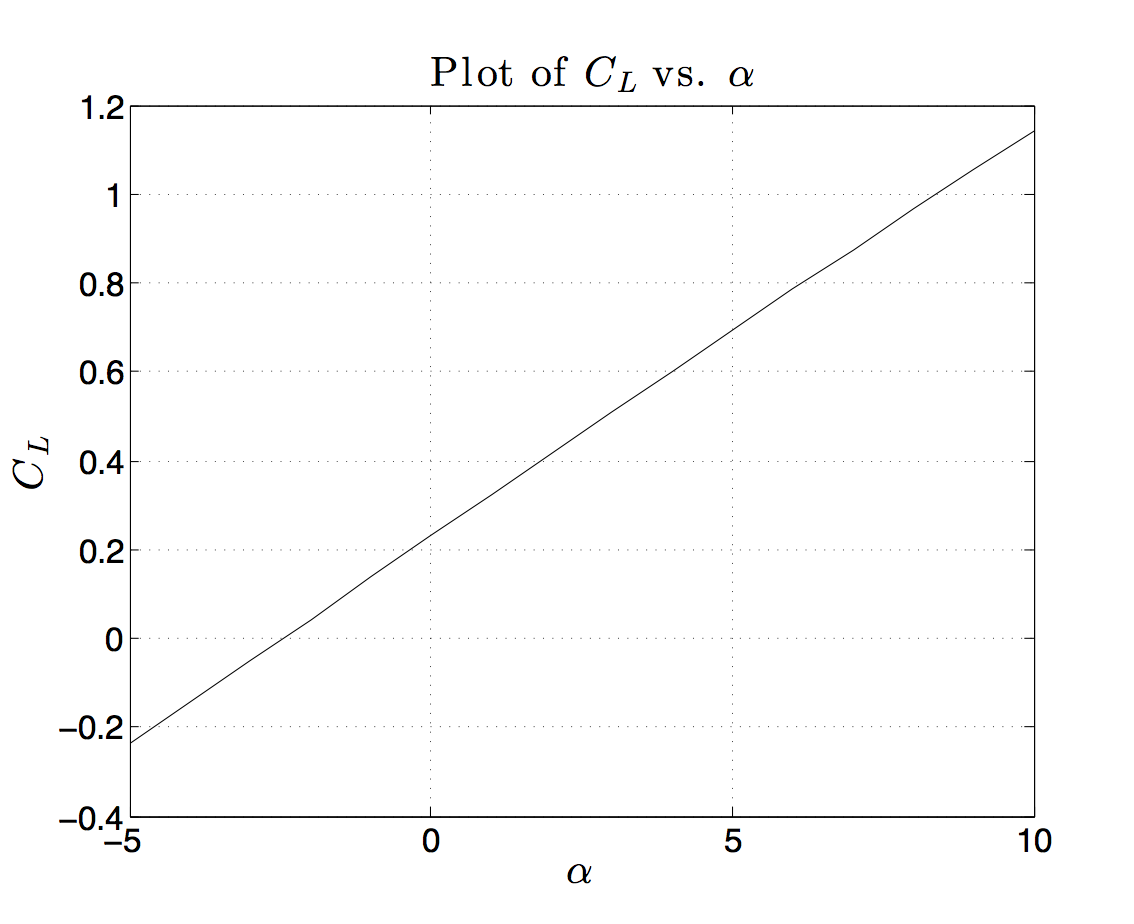
\includegraphics[width=0.7\textwidth]{Figures/PS3/CL_vs_alpha.png}
    	\caption{$C_L$ vs $\alpha$}\label{fig:cl-alpha}
    \end{figure}
    \begin{figure}[h!]
    	\centering
    	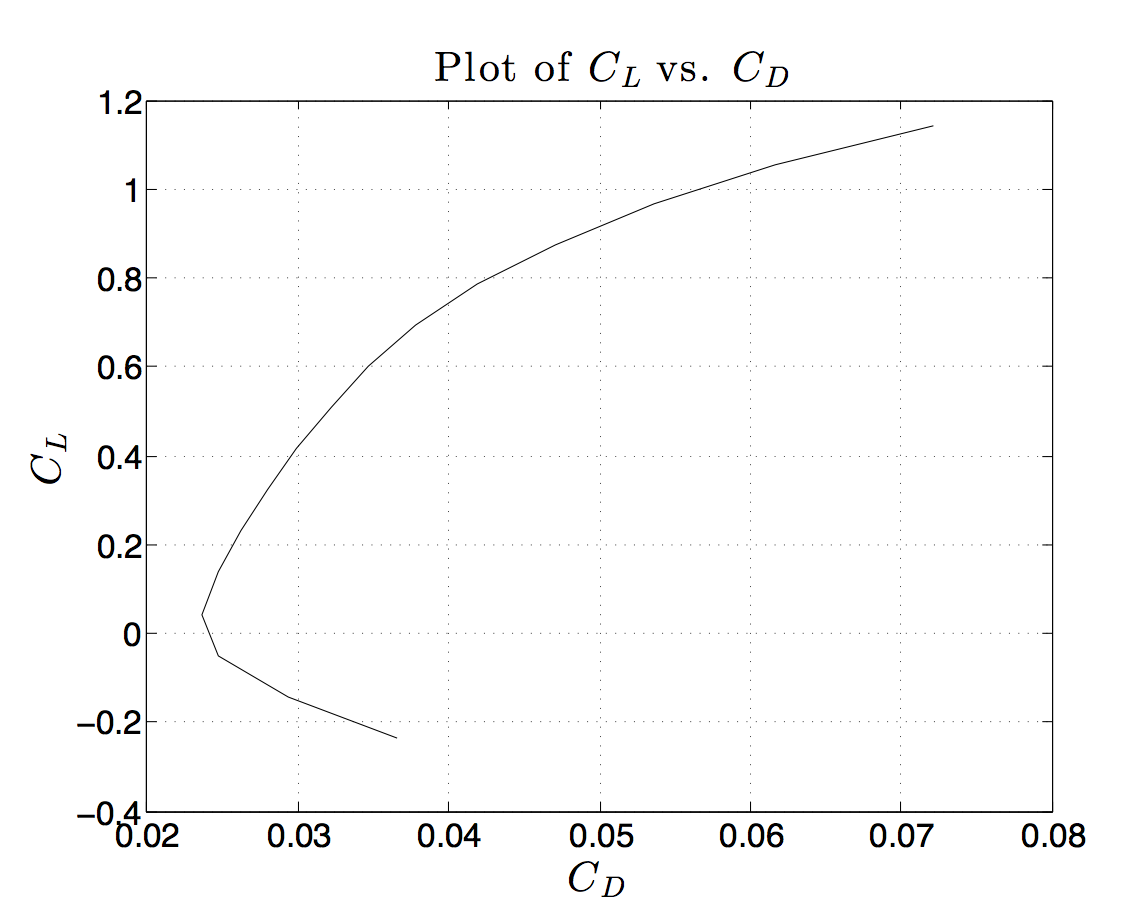
\includegraphics[width=0.7\textwidth]{Figures/PS3/CL_vs_CD.png}
    	\caption{Drag polar}\label{fig:cl-cd}
    \end{figure}
    \begin{figure}[h!]
    	\centering
    	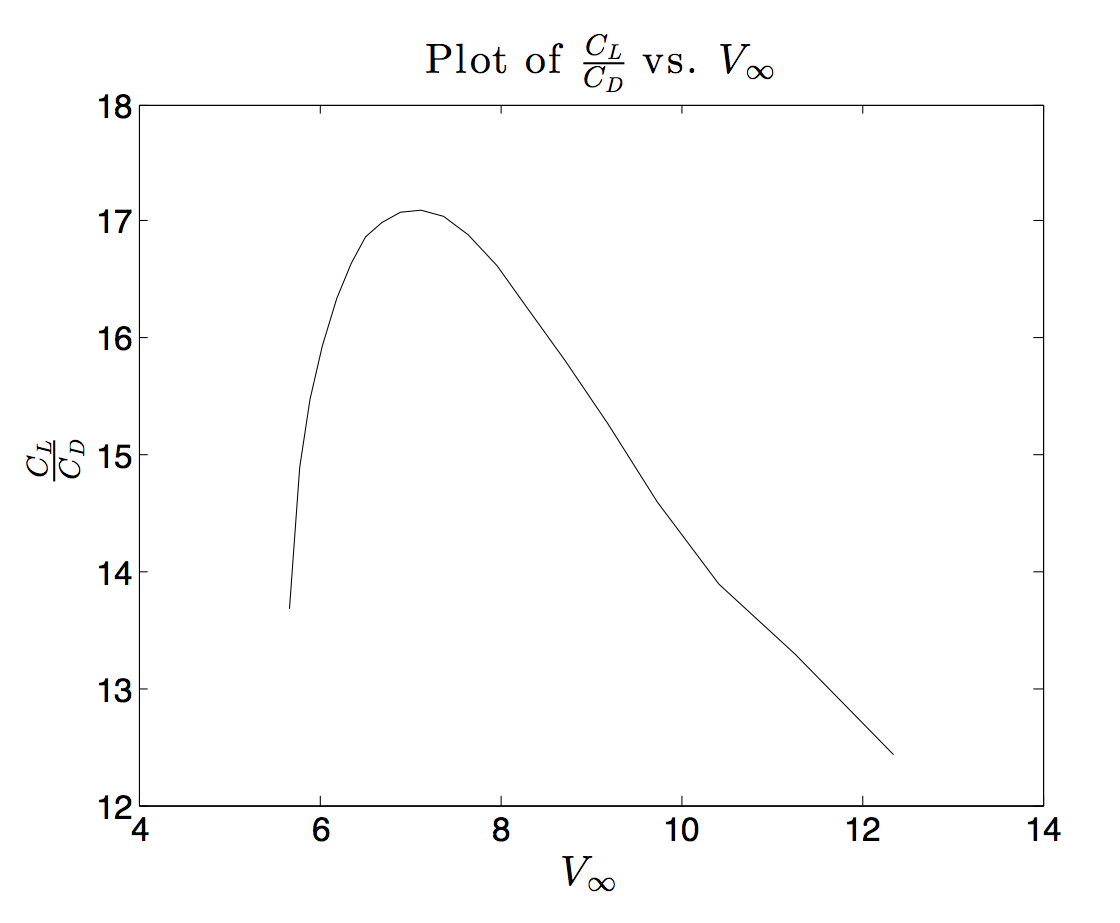
\includegraphics[width=0.7\textwidth]{Figures/PS3/CL-CD_vs_V.png}
    	\caption{$C_L/C_D$ vs $v_\infty$}\label{fig:LD-v}
    \end{figure}
    \begin{figure}[h!]
    	\centering
    	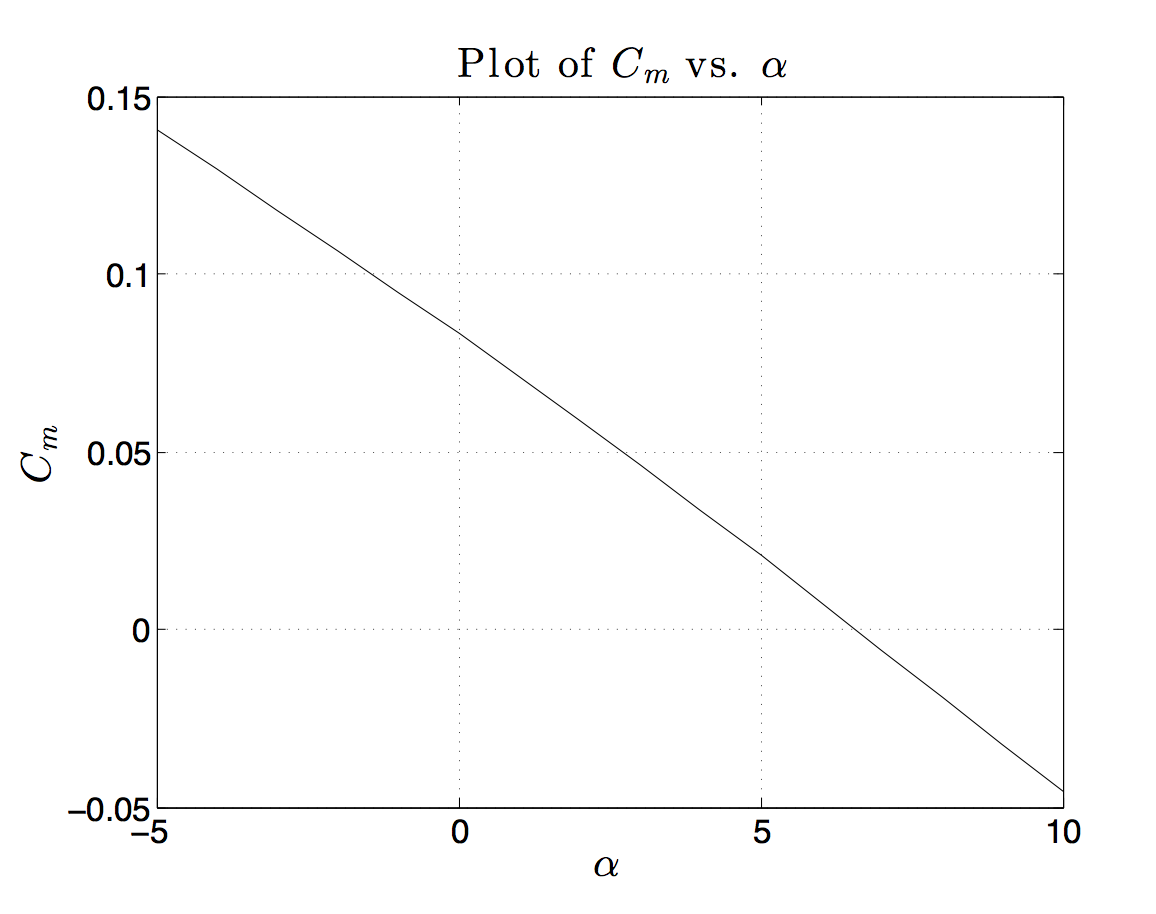
\includegraphics[width=0.7\textwidth]{Figures/PS3/Cm_vs_alpha.png}
    	\caption{$C_m$ vs $\alpha$}\label{fig:cm-alpha}
    \end{figure}
    \begin{figure}[h!]
    	\centering
    	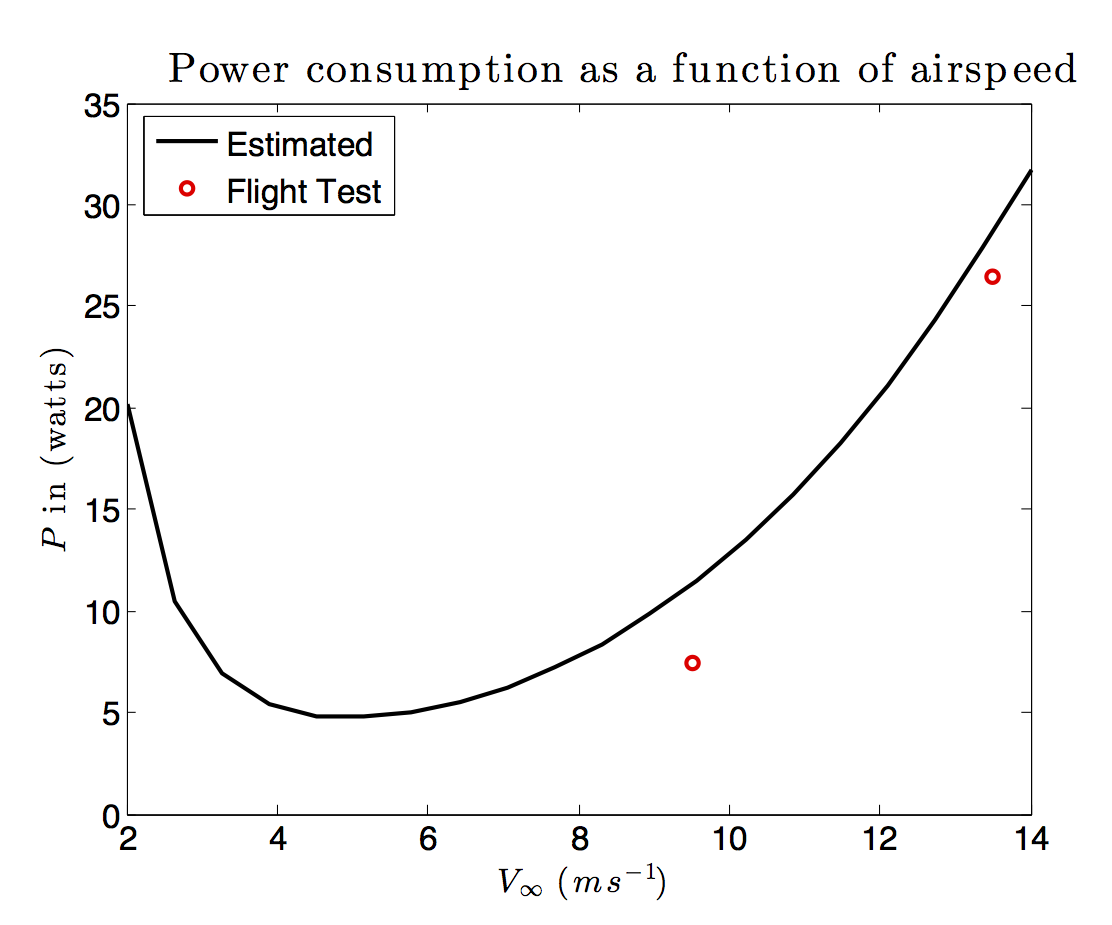
\includegraphics[width=0.7\textwidth]{Figures/PS3/power_consumption.png}
    	\caption{$P_{level}$ vs airspeed}\label{fig:power-cons}
    \end{figure}

    A comparison of the performance parameters estimated from our analysis with the performance parameters obtained from measured data during flight tests in shown in Table~\ref{table:Compar}.

    \begin{table}[htb]
    	\begin{center}
    		\begin{tabular}{|c|c|c|c|c|c|}
    			\hline
    			\textbf{} & \textbf{$C_L\;max$} & \textbf{$(L/D)_{max}$} & \textbf{$P_{level}$ $(9.5 \; ms^{-1})$} & $P_{level}$ $(13.5 \; ms^{-1})$  & \textbf{$P_{max\;climb}$} \\ 
    			\hline
    			\textbf{Estimated} & $1.14$ & $19.0$ & $11.29\;watts$ & $28.62\;watts$ & $34.12\;watts$  \\
    			\textbf{Measured}  & $0.73$ & $16.3$ & $7.45\;watts$ & $26.47\;watts$ & $39.98\;watts$  \\
    			\hline
    		\end{tabular}
    	\end{center}
    	\caption{Estimated vs. measured flight performance parameters}
    	\label{table:Compar} 
    \end{table}

    \subsection{Stability Analysis}

    The stability analysis of our design was performed in AVL. Three different straight and level flight trim states and one level turn trim state were analysed. The four cases used are listed in Table~\ref{table:stab-cases}.

    \begin{table}[htb]
    	\begin{center}
    		\begin{tabular}{|c|c|c|}
    			\hline
    			\textbf{Case} & \textbf{Airspeed (in m/s)} & \textbf{Bank Angle (in degrees)} \\ 
    			\hline
    			Case 1 &  $8.5$ &  $0$ \\
    			Case 2 &  $7.0$ &  $0$ \\
    			Case 3 & $10.0$ &  $0$ \\
    			Case 4 &  $8.5$ & $30$ \\
    			\hline
    		\end{tabular}
    	\end{center}
    	\caption{Different cases for stability analysis in AVL}
    	\label{table:stab-cases} 
    \end{table}

    The eigenvalues, frequencies and damping ratios for the different modes are plotted in Figures~\ref{fig:eig},~\ref{fig:freq} and \ref{fig:damp}.

    \begin{figure}[h!]
    	\centering
    	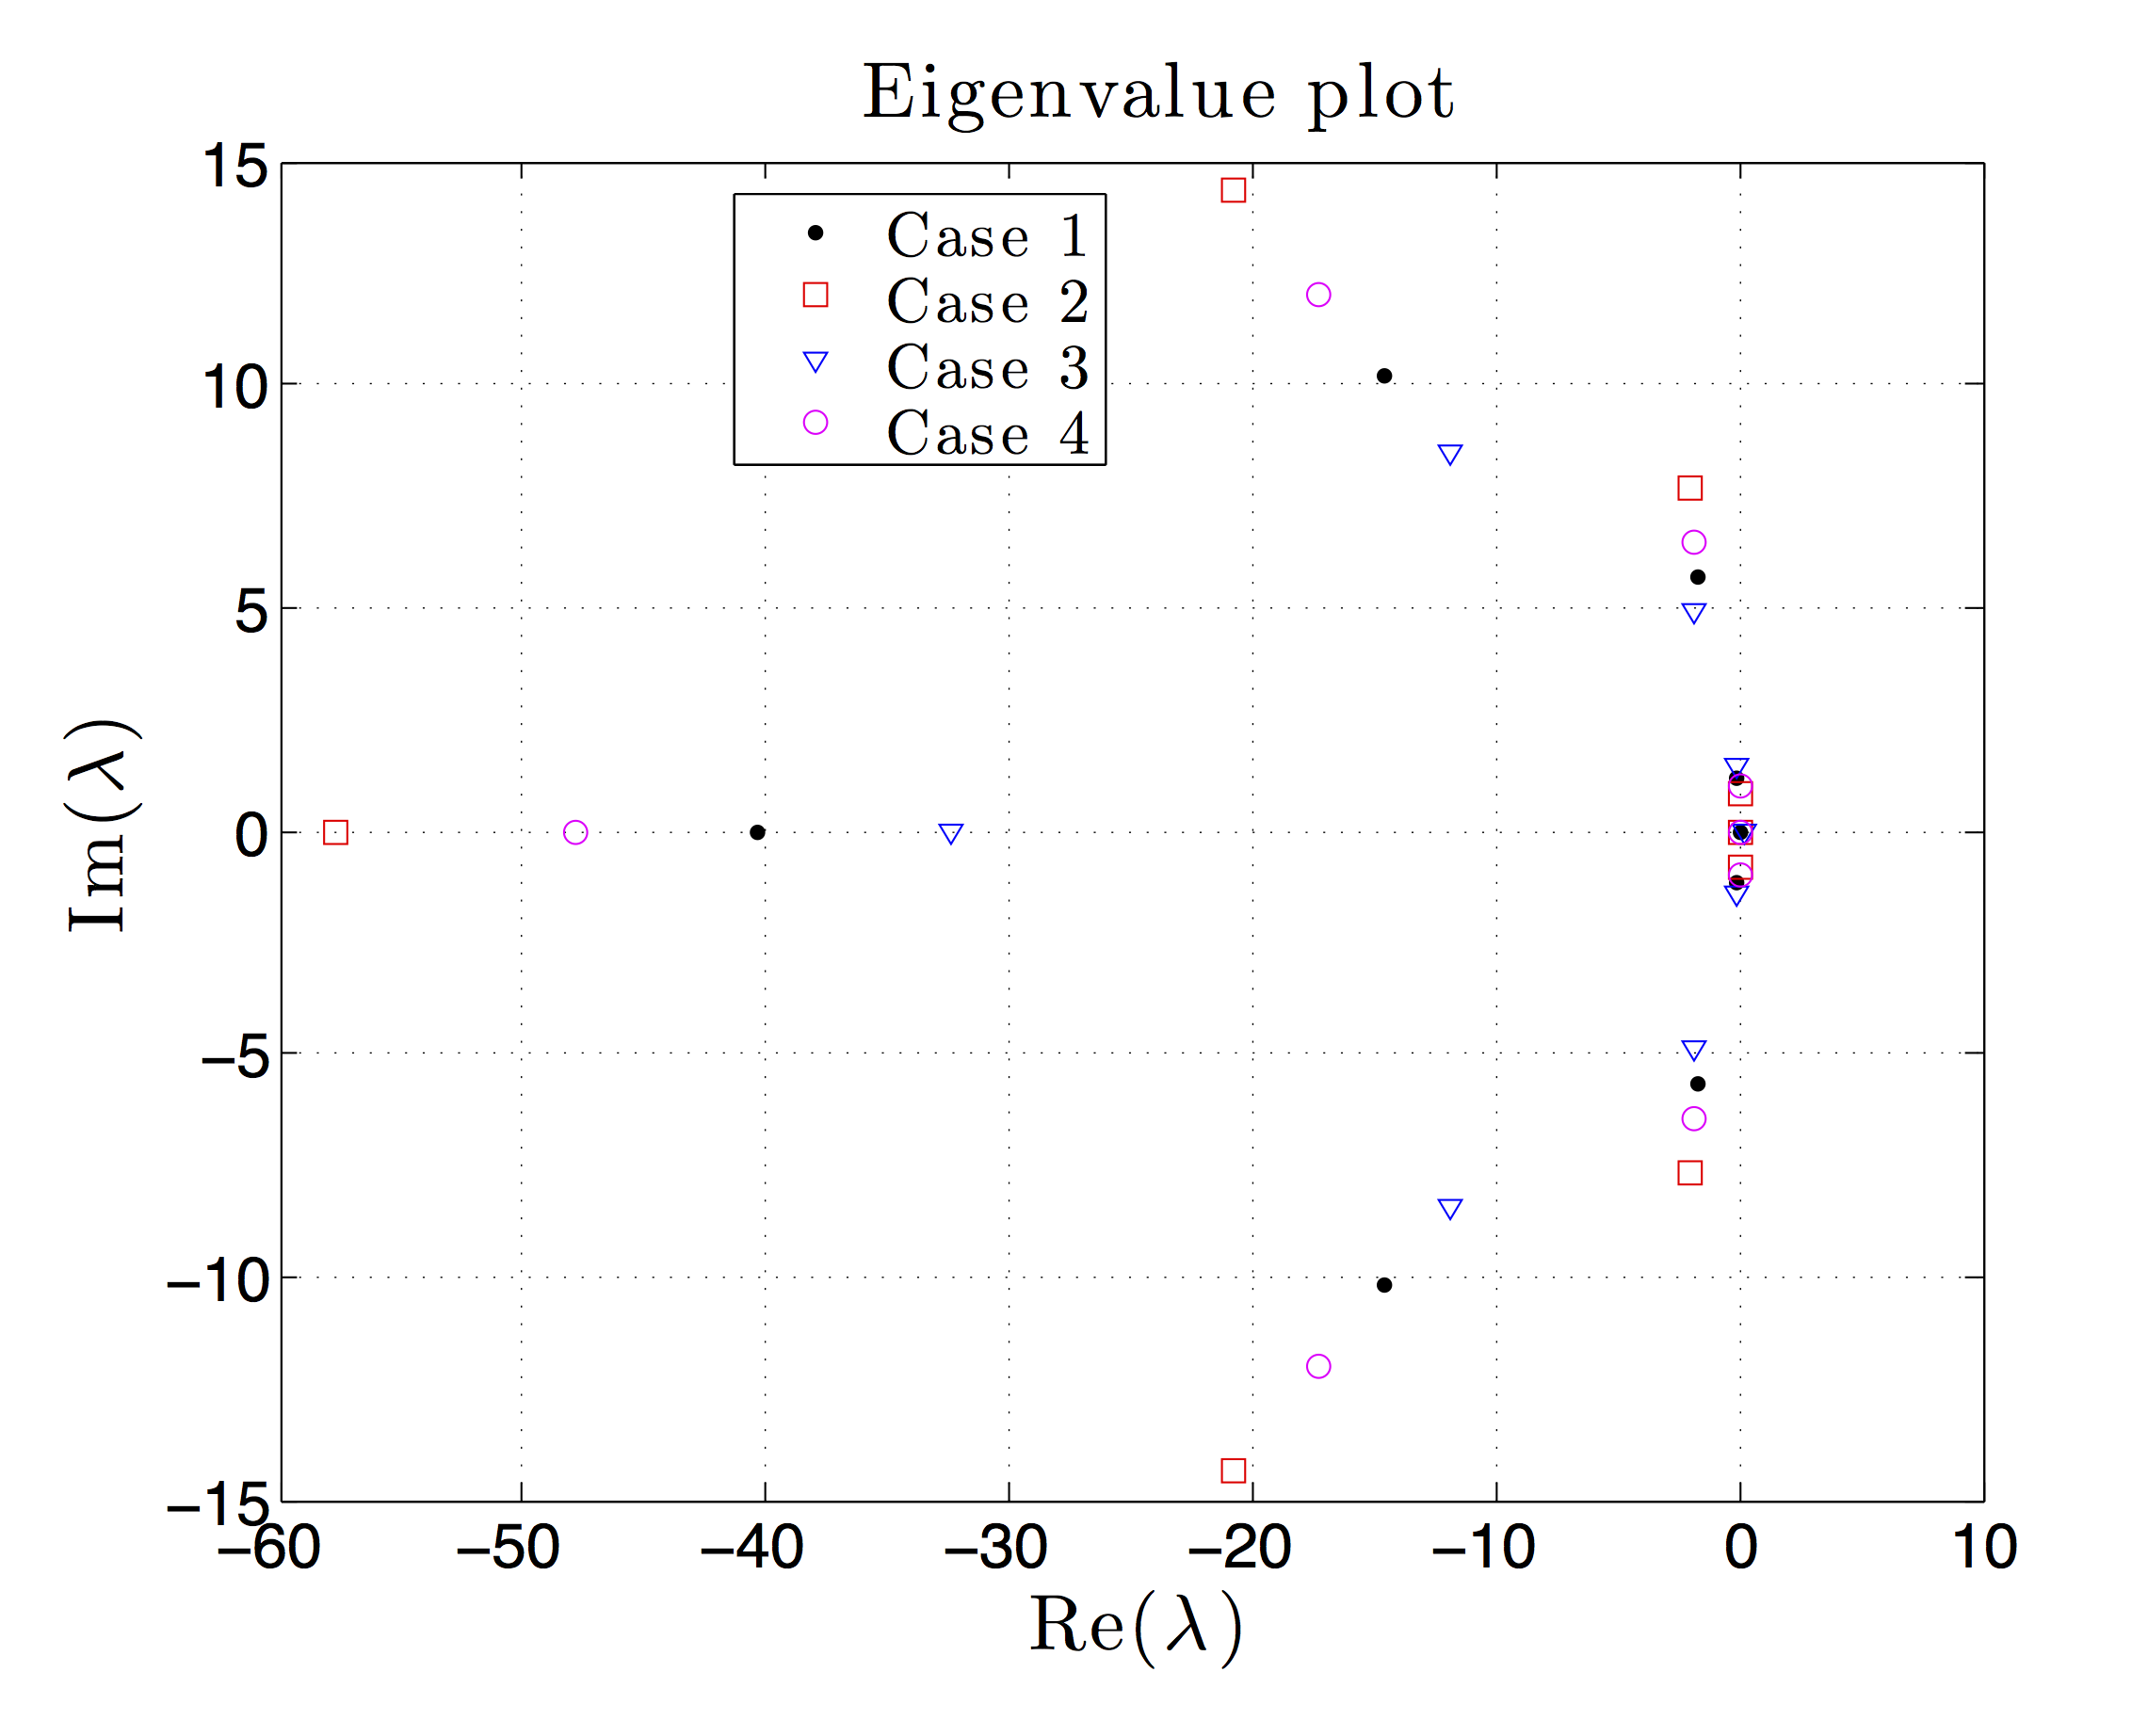
\includegraphics[width=0.7\textwidth]{Figures/PS2/SkynetV1_eig.png}
    	\caption{Eigenvalue plot}\label{fig:eig}
    \end{figure}
    \begin{figure}[h!]
    	\centering
    	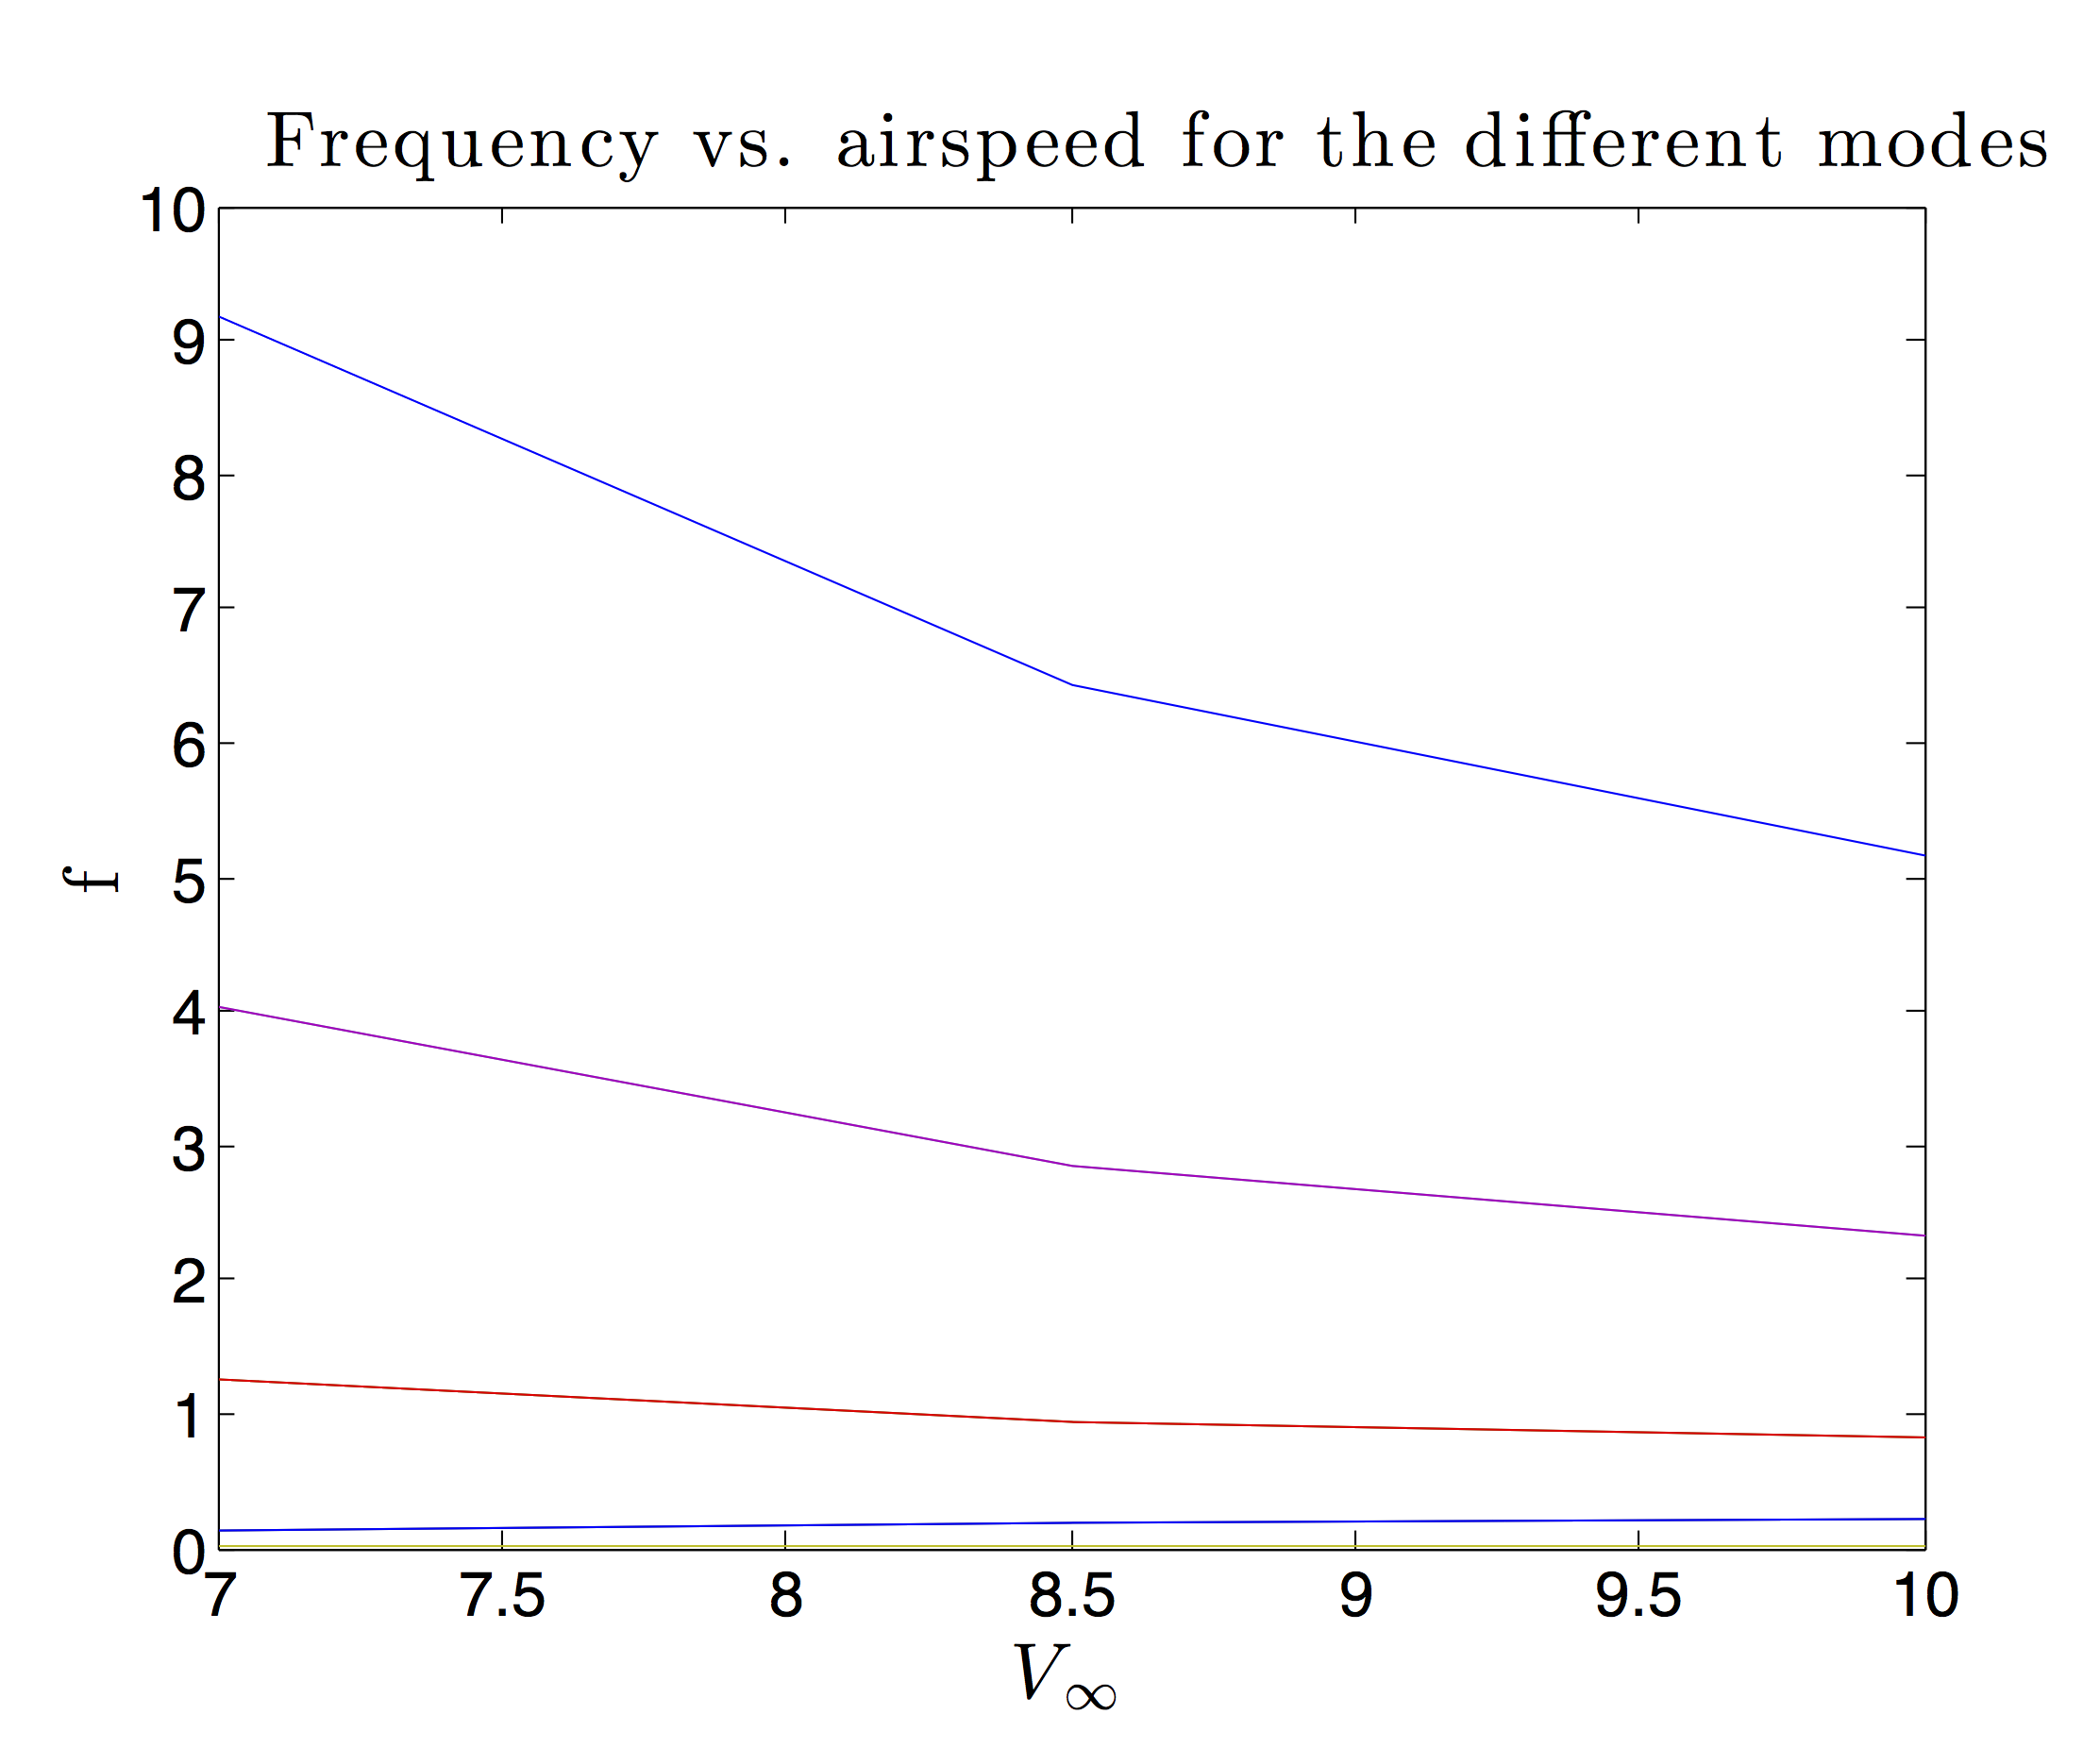
\includegraphics[width=0.7\textwidth]{Figures/PS2/SkynetV1_freq.png}
    	\caption{Frequency}\label{fig:freq}
    \end{figure}
    \begin{figure}[h!]
    	\centering
    	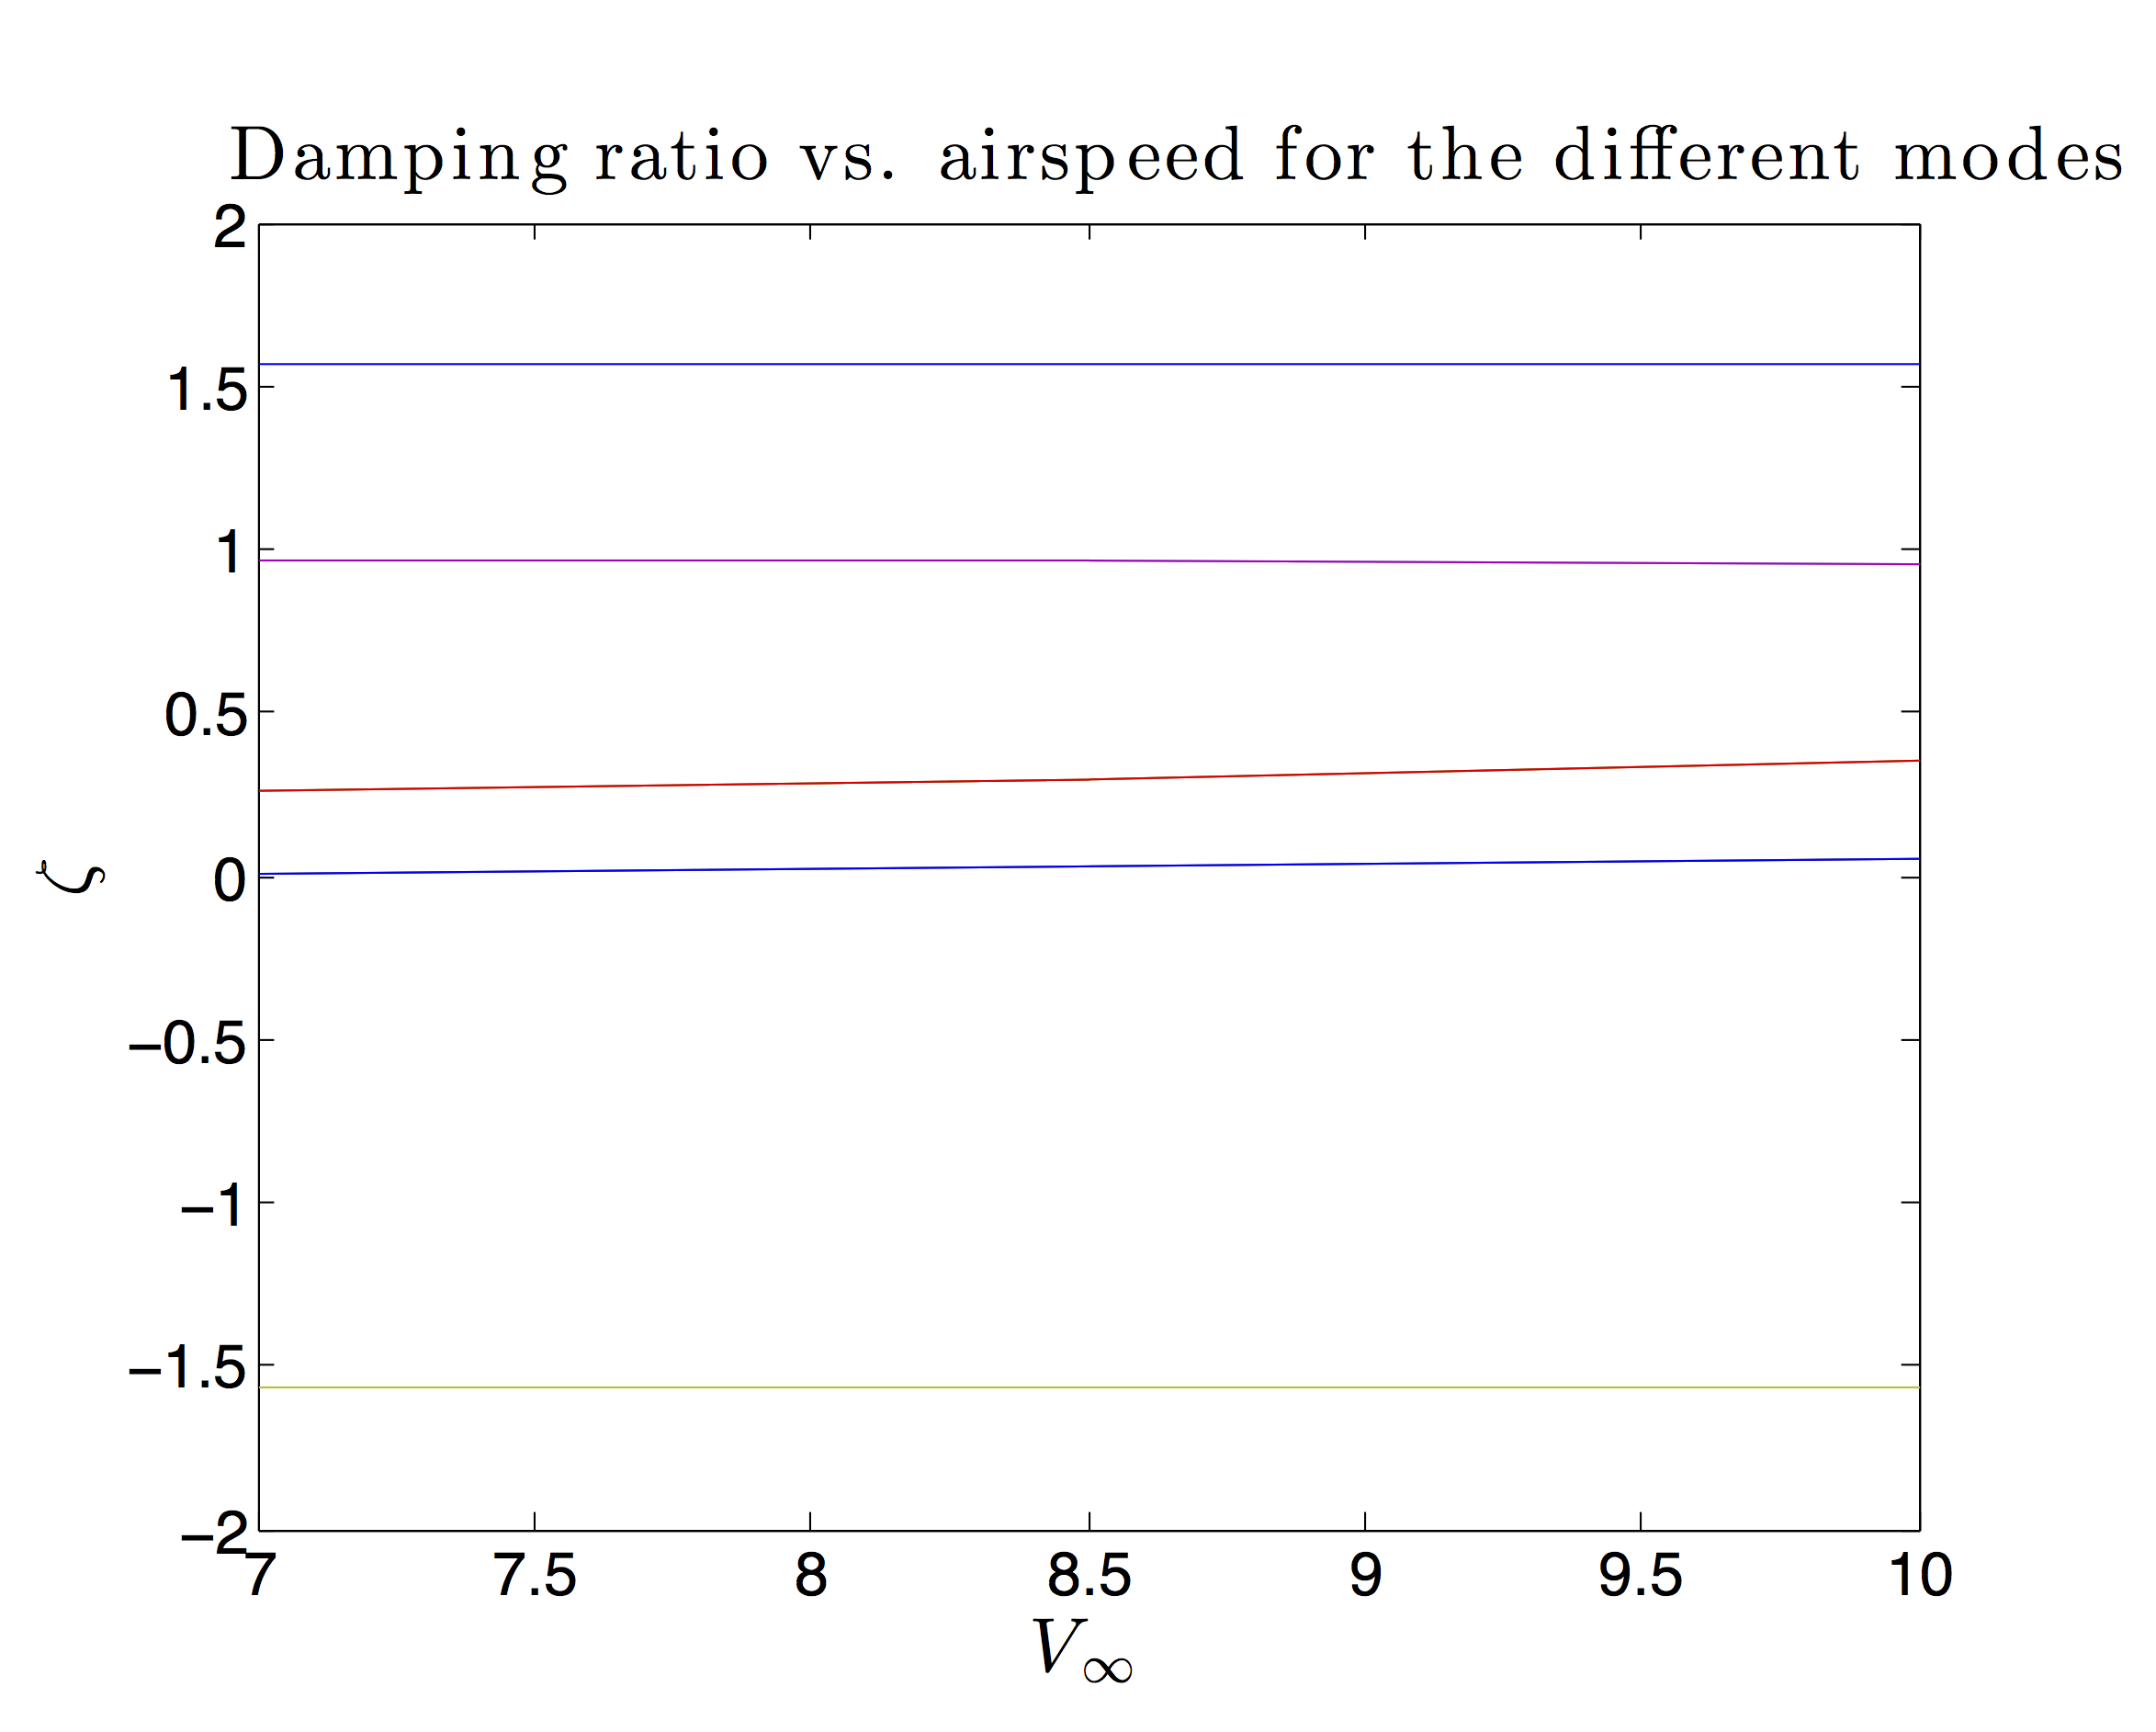
\includegraphics[width=0.7\textwidth]{Figures/PS2/SkynetV1_damp.png}
    	\caption{Damping ratio}\label{fig:damp}
    \end{figure}

    \subsection{Three-view drawings of the final design}

    Figure~\ref{fig:CAD} shows the CAD drawings of our final design. Figure~\ref{fig:SW} shows the SolidWorks model of our design that we used to get all the parts for the laser cutter.

    \begin{figure}[h!]
    	\centering
    	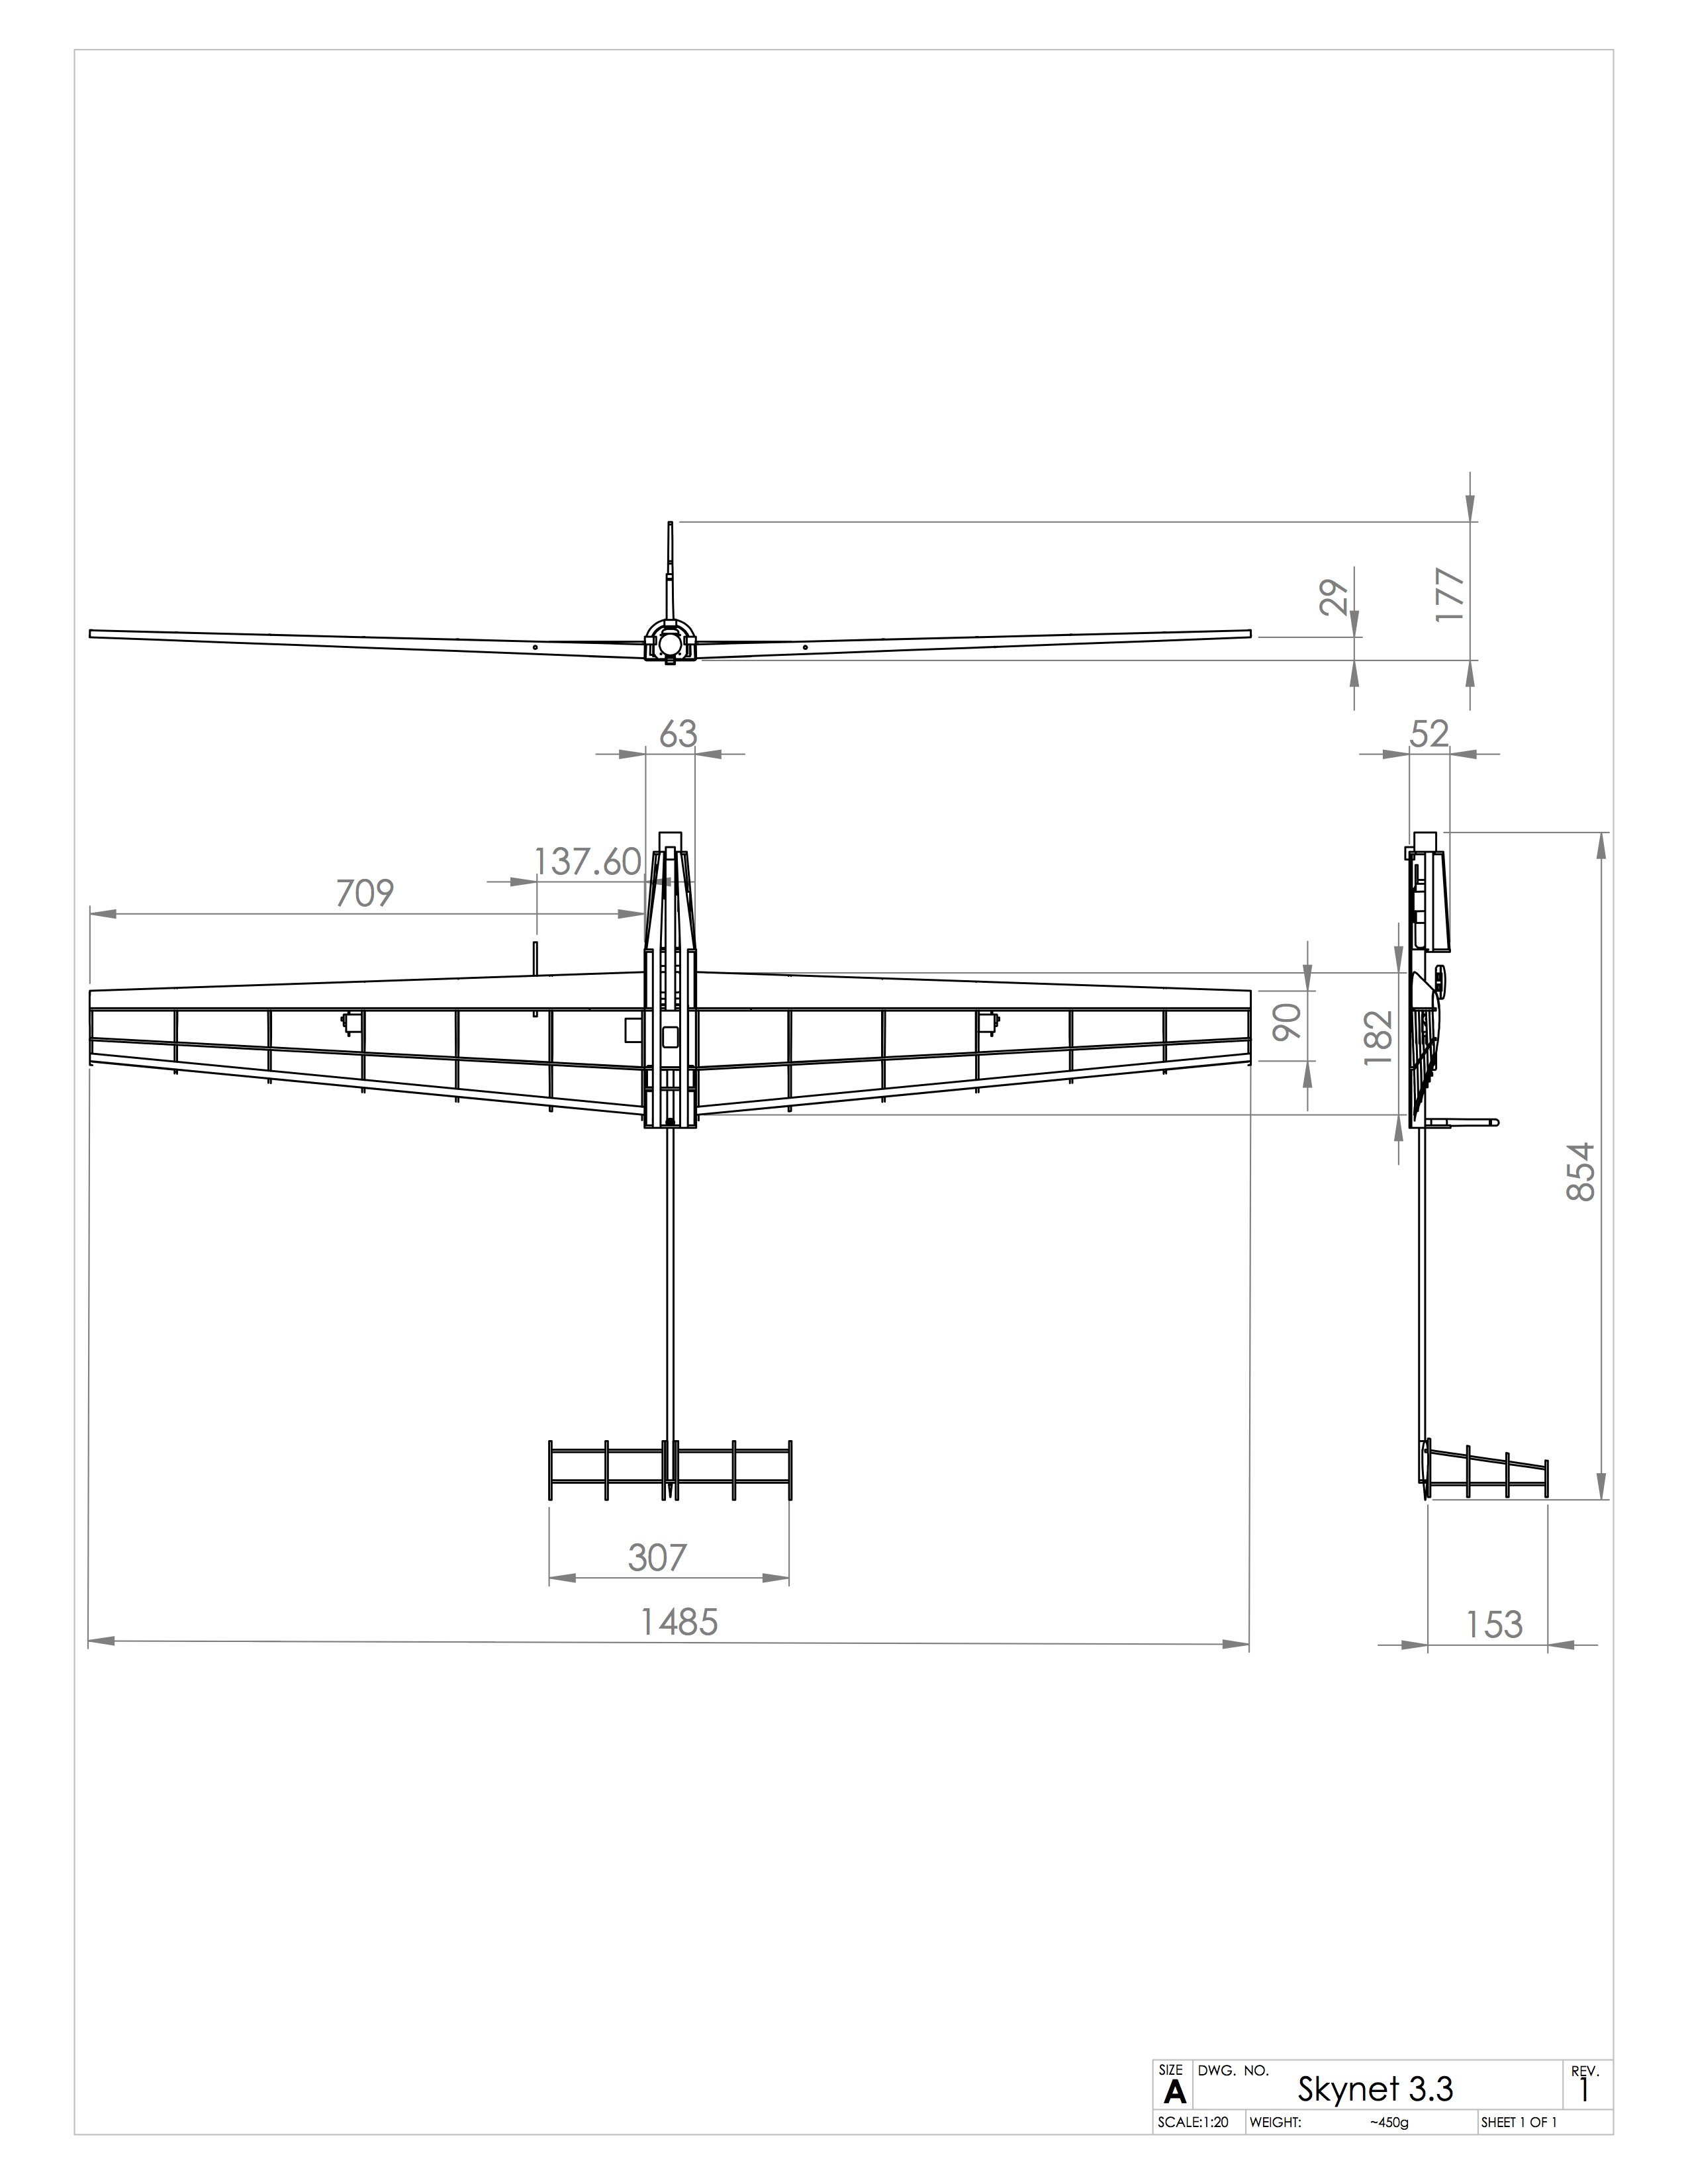
\includegraphics[width=\textwidth]{Figures/CAD/Aircraft_Design_3-3.png}
    	\caption{CAD drawings of the final design}\label{fig:CAD}
    \end{figure}

    \begin{figure}[h!]
    	\centering
    	\begin{subfigure}[b]{0.49\textwidth}
    		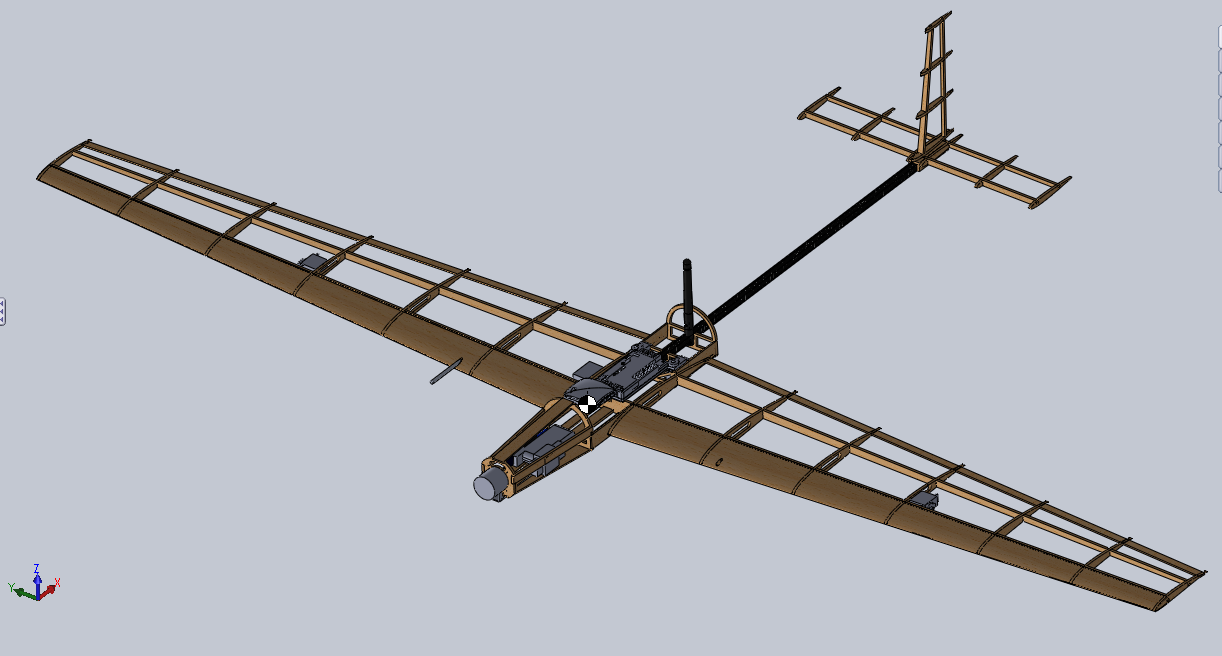
\includegraphics[width=\textwidth]{Figures/CAD/iso.png}
    		\caption{Isometric view}
    	\end{subfigure}
    	\begin{subfigure}[b]{0.49\textwidth}
    		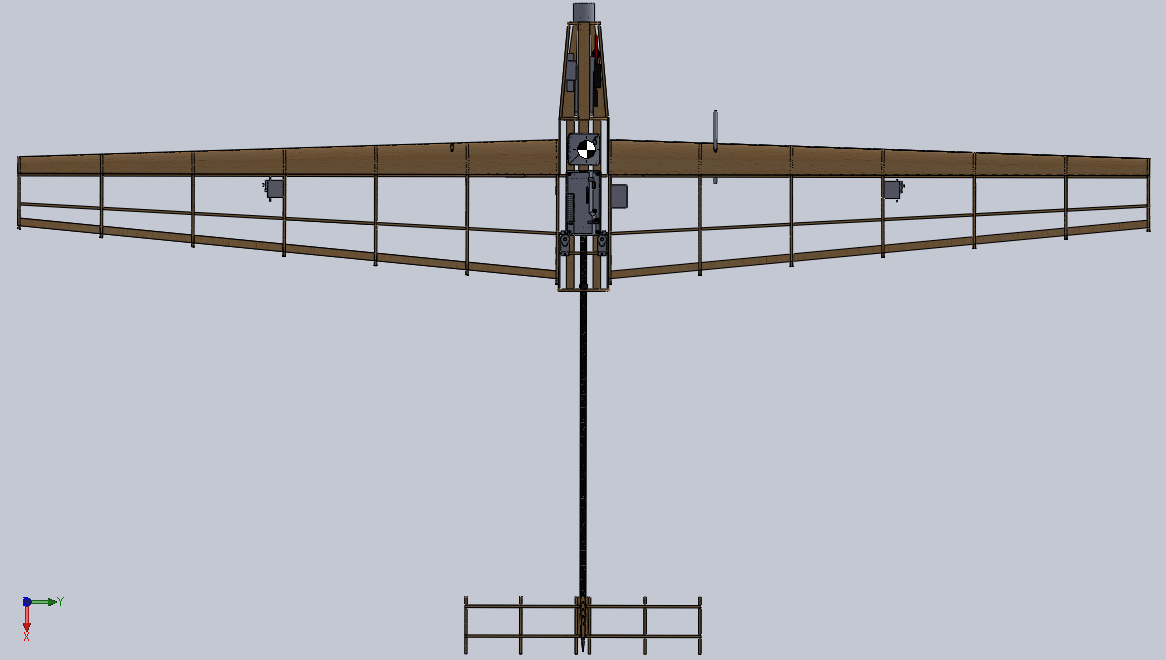
\includegraphics[width=\textwidth]{Figures/CAD/top.png}
    		\caption{Top view}
    	\end{subfigure}
    	\\
    	\begin{subfigure}[b]{0.49\textwidth}
    		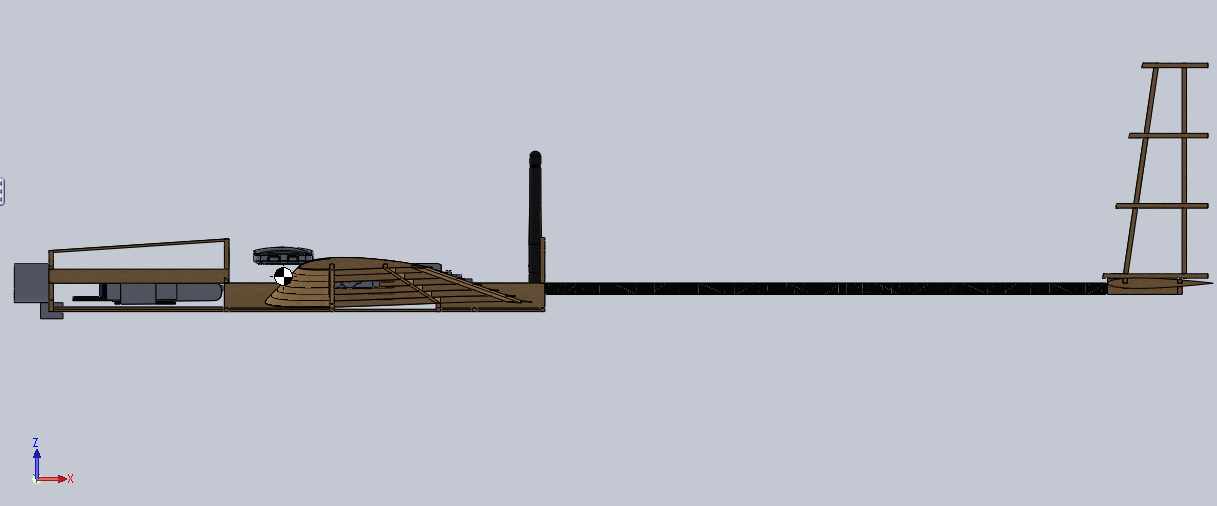
\includegraphics[width=\textwidth]{Figures/CAD/side.png}
    		\caption{Side view}
    	\end{subfigure}
    	\begin{subfigure}[b]{0.49\textwidth}
    		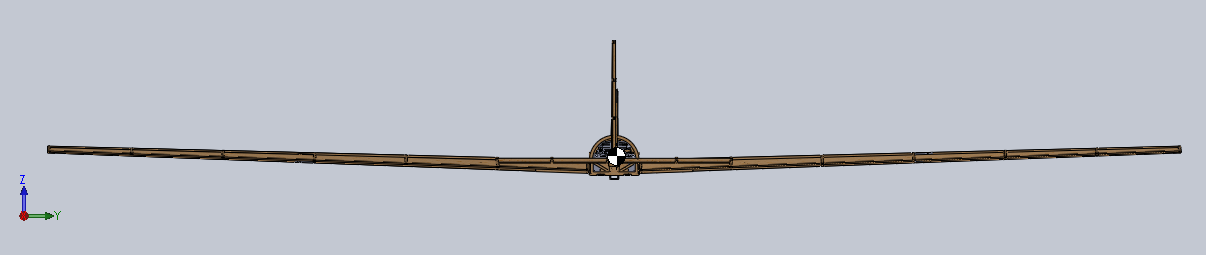
\includegraphics[width=\textwidth]{Figures/CAD/front.png}
    		\caption{Front view}
        \end{subfigure}%
        \caption{Solidworks model screenshots}\label{fig:SW}
    \end{figure}

\FloatBarrier
\section{Controls}
\label{Controls}
\subsection{Control Strategy}
\label{CtrlStr}

The controller for the aircraft used successive loop closure to obtain the closed loop performance necessary to complete our missions. The strategy was to provide the navigation team with a robust interface that they could use to carry out the mission. This interface sectioned off the inner loop controls from the outer loop / guidance and navigation controls. The interface that the navigation team had to work with was commanded ground speed, commanded heading, and commanded altitude. These three references were used dynamically by the navigation team to carry out our complete mission.

Waypoint navigation was obtained by commanding heading, ground speed, and altitude in the medium (10 Hz) AUTO loop. The inner loop controllers ran at within the 50 Hz loop to maintain the commanded heading, ground speed, and altitude. This interface was the most important, and most difficult to realize in order to accomplish the relatively complex mission profile.

\paragraph{Inner Loop Controllers}
The inner most controllers consisted of three PID loops to command throttle, elevator deflection, and aileron deflection. To obtain the correct airspeed, a throttle scheduler was used as a feedforward term to overcome the nonlinearities in the throttle command over the aircraft's airspeed envelope. For the pitch and roll controllers, simple PI control sufficed.

\begin{figure}[h!]
\centering
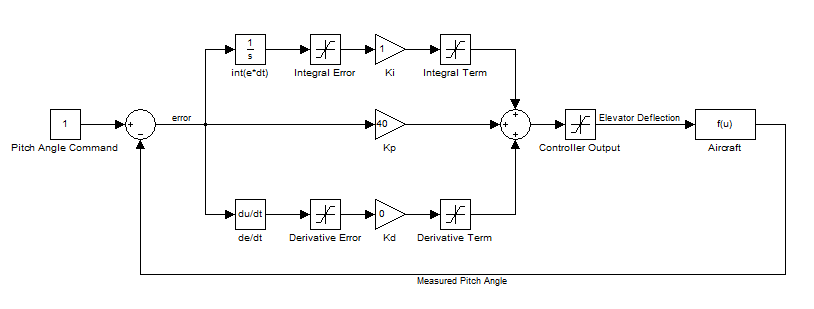
\includegraphics[width=\textwidth]{./Figures/PitchAngleController}
\caption{Pitch Angle Controller}
\label{fig:PitchAngleController}
\end{figure}

\begin{figure}[h!]
\centering
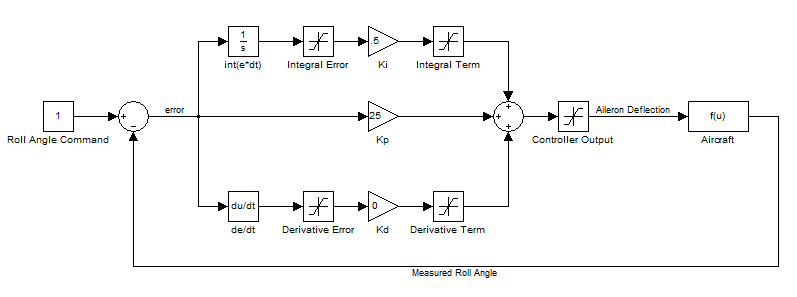
\includegraphics[width=\textwidth]{./Figures/RollAngleController}
\caption{Roll Angle Controller}
\label{fig:RollAngleController}
\end{figure}

\begin{figure}[h!]
\centering
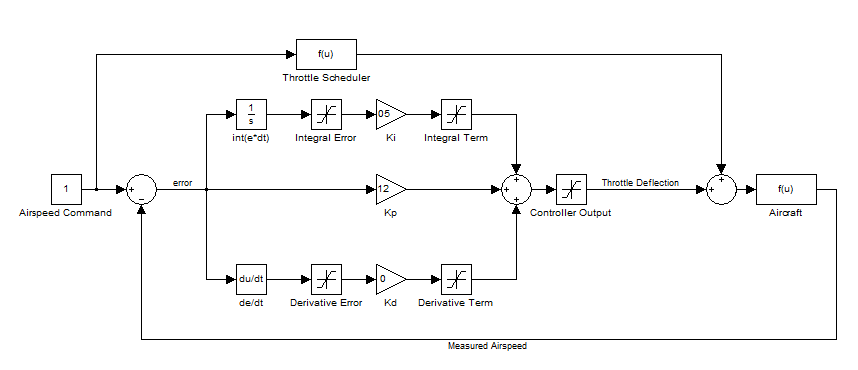
\includegraphics[width=\textwidth]{./Figures/AirspeedController}
\caption{Airspeed Controller}
\label{fig:AirspeedController}
\end{figure}

The altitude controller relied on the ability of the airspeed controller to maintain a relatively constant airspeed even with disturbances due to wind, roll angle changes, and pitch angle changes in the aircraft. Trim states for steady level flight, 15 degree roll turns, and 30 degree roll turns were determined experimentally across the entire airspeed envelope of 8.5 m/s to 13.5 m/s. Once the trim state altitude holding states were known, the pitch angle scheduler was built using switch case statements and a discretized state space of the airspeed and roll angle commands. The altitude controller relied heavily on the scheduler and only allowed small perturbations in pitch angle to maintain the altitude. The limiters on this controller in particular were too restrictive to begin with and therefore in windy conditions, the controller did not have enough authority to maintain constant altitude.

\begin{figure}[h!]
\centering
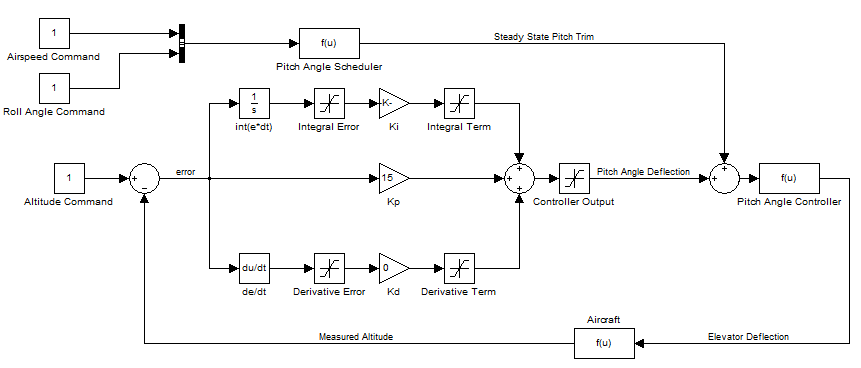
\includegraphics[width=\textwidth]{./Figures/AltitudeController}
\caption{Altitude Controller}
\label{fig:AltitudeController}
\end{figure}

The heading controller looped around the roll angle controller to provide the navigation team with heading command tracking. The heading controller was the only controller to use full PID control in order to dampen the oscillations of heading hold / heading tracking at low airspeeds. The introduction of derivative term control was key in gaining robustness in the controller during the refinement phase of our mission at the low (sub 9 m/s) airspeeds.

\begin{figure}[h!]
\centering
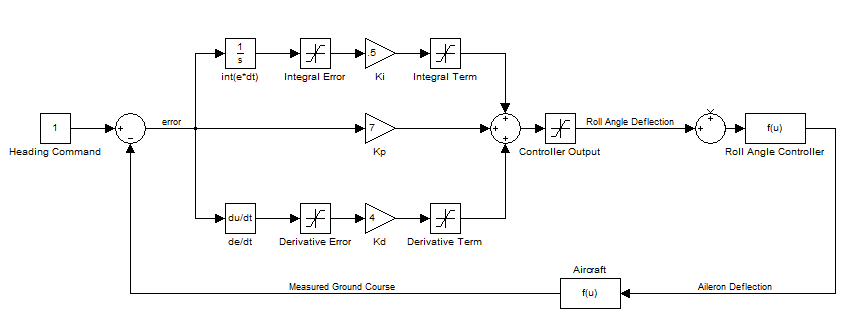
\includegraphics[width=\textwidth]{./Figures/HeadingController}
\caption{Heading Controller}
\label{fig:HeadingController}
\end{figure}

The last of the inner loop controllers to be used to provide the complete interface for the navigation team was the ground speed controller. This controller took a ground speed reference that was dynamically updating from the mission management and commanded an airspeed for the airspeed controller to track. In reality, we never really got around to dynamically changing the ground speed and simply opted to maintain a single ground speed in the first phase of the mission and a second (slower) ground speed during the second phase of the mission.

\begin{figure}[h!]
\centering
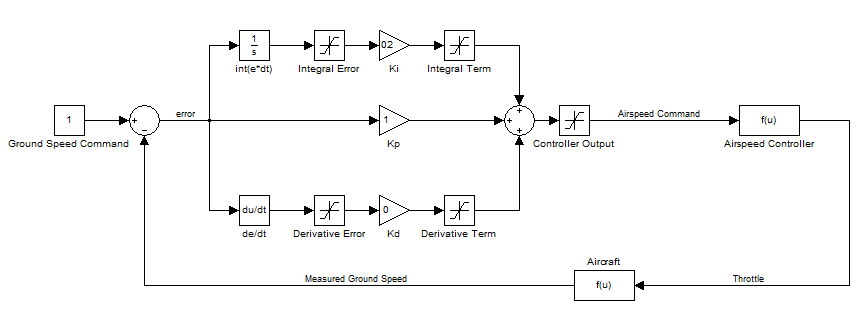
\includegraphics[width=\textwidth]{./Figures/GroundSpeedController}
\caption{Ground Speed Controller}
\label{fig:GroundSpeedController}
\end{figure}

\subsection{Flight Performance}
\label{CtrlFlightPerf}
% BRANDON
% Include in this section Initial Approach vs. Final Choices

The successive loop strategy worked well for the job that was required by our mission plan. Experimental results were almost always needed in order to tune the gains for each individual controller and an extensive steady state level flight / banked constant altitude set of experiments led to the trim schedulers needed. The initial plan for controller design was to use a quick successive loop closure controller for the preliminary problem sets and migrate to a linear quadratic regulator eventually. The quick controller was programmed in C++ and ready for testing several weeks prior to the line tracking problem set. However, our team ran up against two road blocks: the first was that we needed CAD models of the aircraft design in order to laser cut the aircraft, the second was that we ran out of flash memory and weren't aware that we could remove much of the APM code to give us more program memory space.

The first issue caused the controller design to halt for about 10-14 days while laser cut prototypes were cut, built, and tested. The second issue caused a complete refactoring of the simple inner loop controls in order to get something flyable as soon as possible. By the time these two issues were resolved, there was no time to continue development on the LQR controller.

\begin{figure}[h!]
\centering
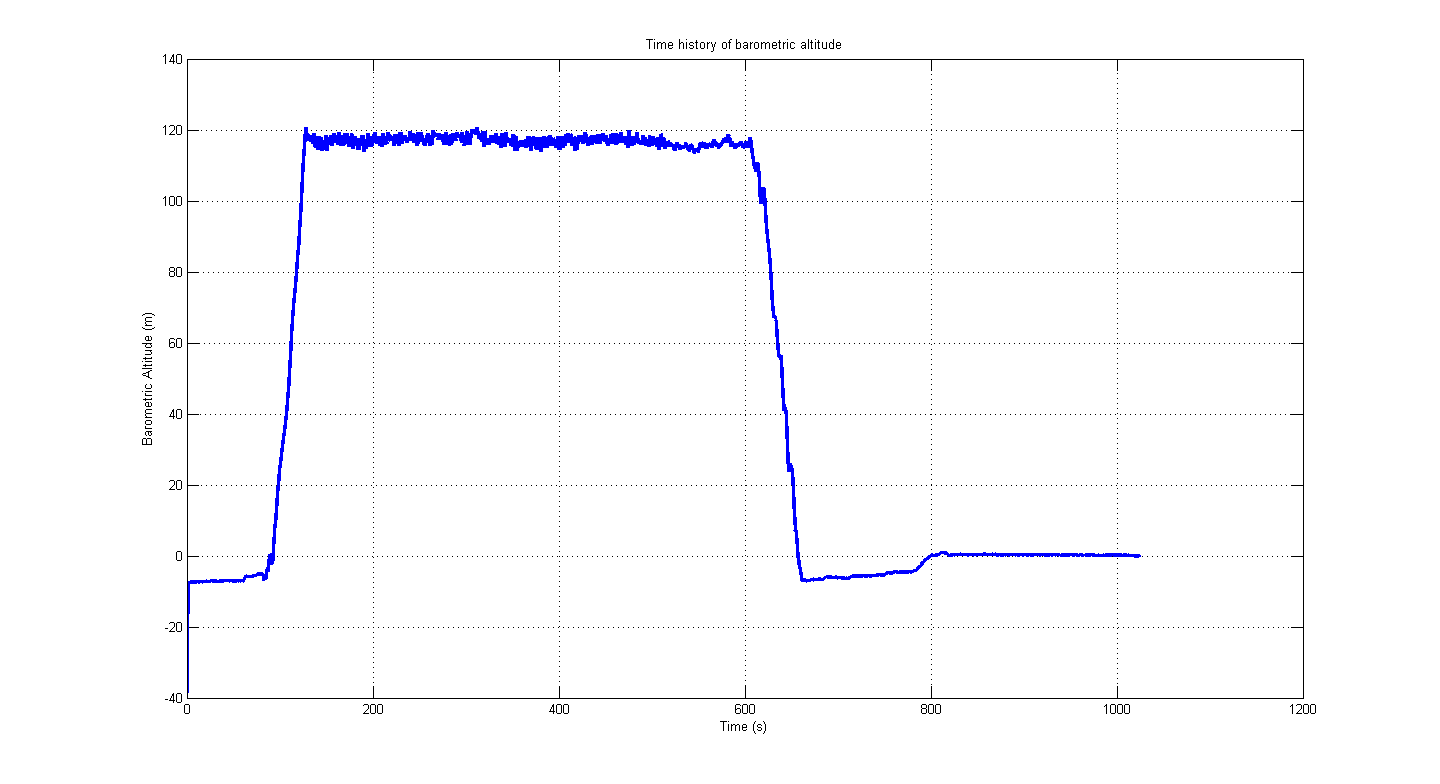
\includegraphics[width=\textwidth]{./Figures/AltitudeHoldPerformance}
\caption{Altitude Hold Performance}
\label{fig:AltitudeHoldPerformance}
\end{figure}

\begin{figure}[h!]
\centering
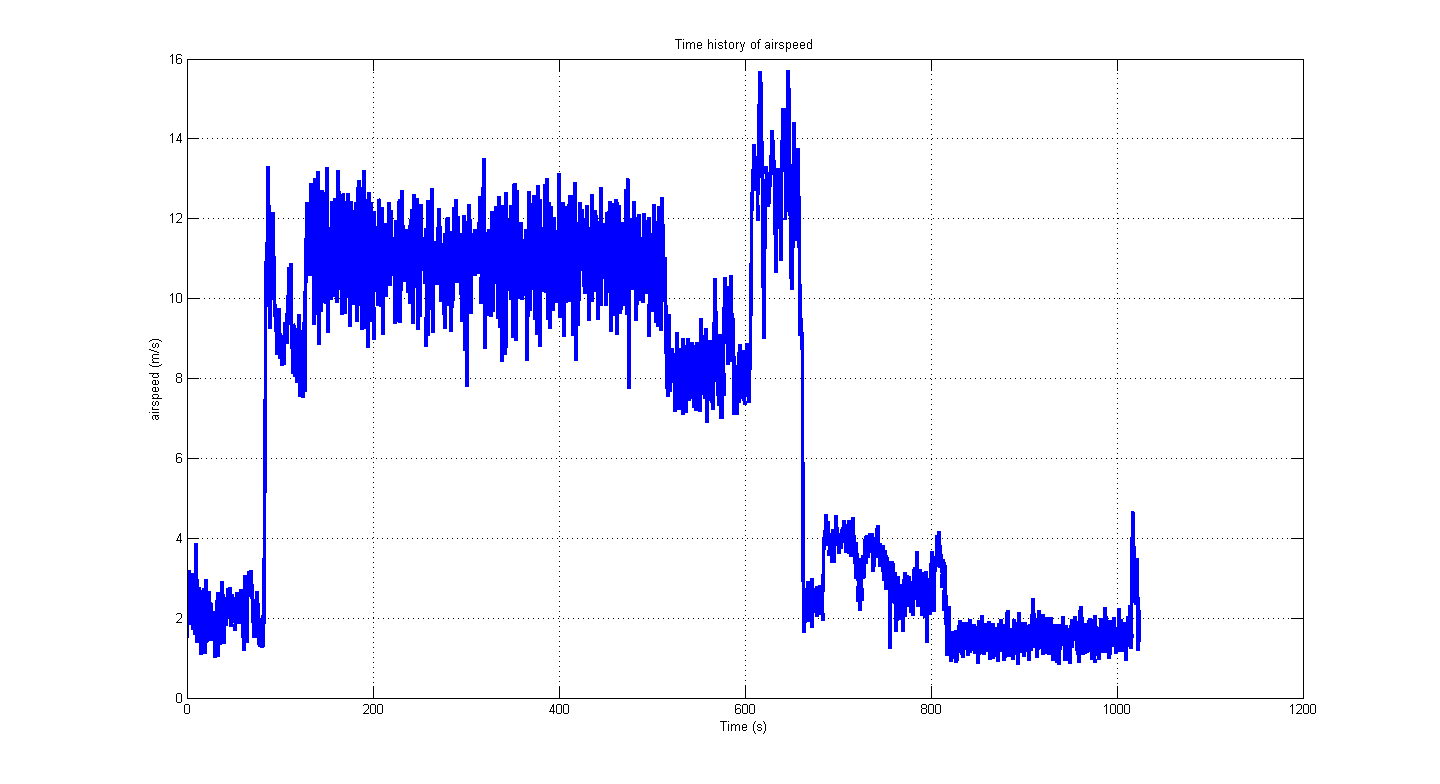
\includegraphics[width=\textwidth]{./Figures/AirspeedHoldPerformance}
\caption{Airspeed Hold Performance}
\label{fig:AirspeedHoldPerformance}
\end{figure}

\begin{figure}[h!]
\centering
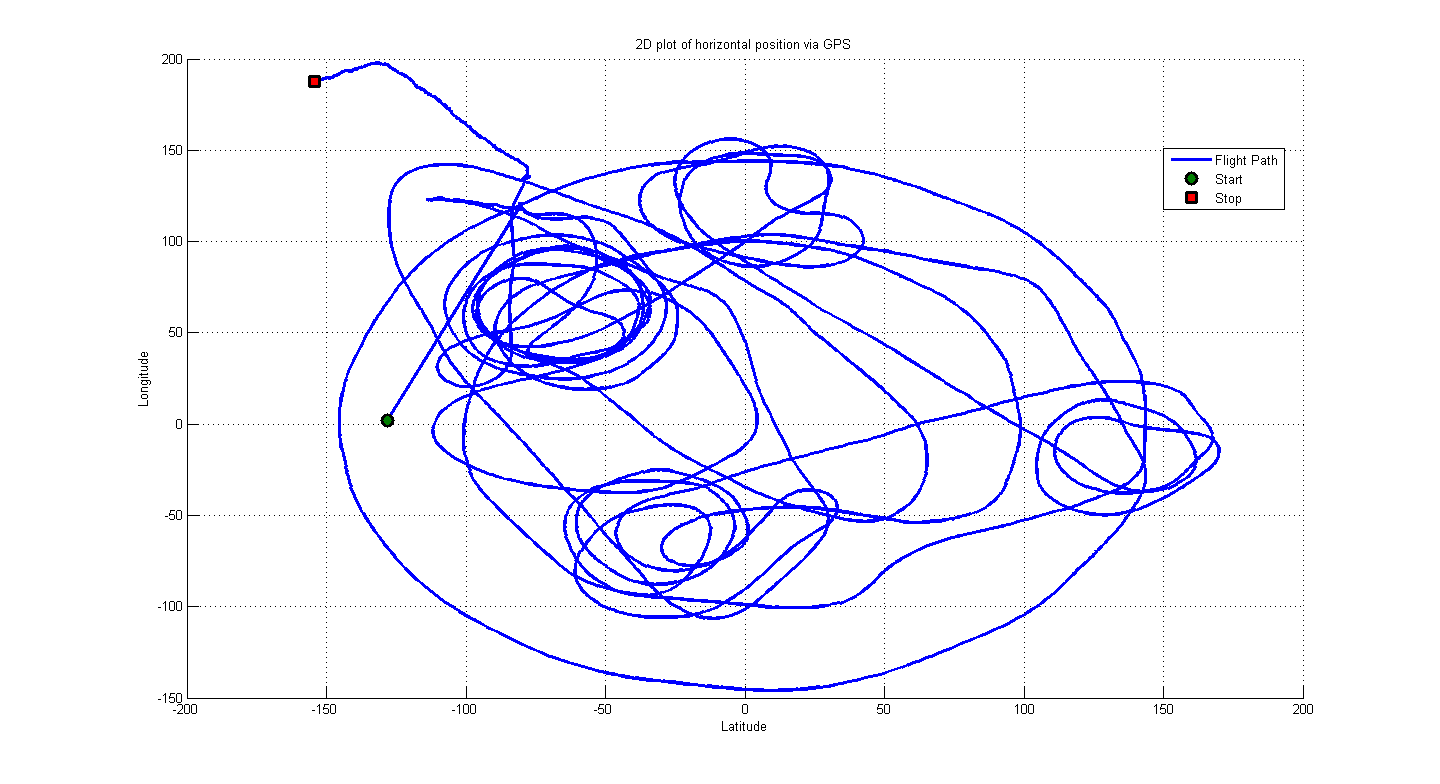
\includegraphics[width=\textwidth]{./Figures/PositionHistory}
\caption{XY Position History}
\label{fig:PositionHistory}
\end{figure}


Figures \ref{fig:AirspeedHoldPerformance} and \ref{fig:AltitudeHoldPerformance} demonstrate the inner loop controllers' ability to hold airspeed and altitude during the mission. The heading control acheived is evidenced by the XY gps position time history of our missions (Figure \ref{fig:PositionHistory}).

\FloatBarrier
\section{Fabrication}
	\label{Fabrication}
	\subsection{Prototype Construction Approach}
	\label{ProtoConsAppr}
	\subsubsection{Mk-I "The Red Baron"}
	\label{mk1}
	\subsubsection{Mk-II "The Pig"}
	\label{mk2}
	\subsubsection{Mk-III.1}
	\label{mk3.1}
	\subsubsection{Mk-III.2 "Ronald McDonald"}
	\label{mk3.2}
	\subsubsection{Mk-III.3 "Terminator"}
	\label{mk3.3}
	\subsubsection{Mk-III.4 "The UltraLight"}
	\label{mk3.4}

%%%%%%%%%%%%%%%% Start: Flight Testing %%%%%%%%%%%%%%%%%%%
\section{Flight Testing}
	\label{FlightTesting}
	Over the course of two weeks, before and during the final competition, the flight test team worked extensively to try to successfully implement the strategies described in section \ref{Mission}. It was decided very early during flight testing that the only way to accomplish the task was to add sections of the mission incrementally. A strategy of "coding at night, flying in the morning" was implemented and each section of the mission was tested in a simulator, tested during flight and gradually changed to improve performance and accommodate realistic goals.

	\subsection{Flight Test Approach}
	\label{FltTstAppr}
	Flight testing was split into three major sections: Waypoint Navigation, Phase 1 testing and Phase 2 testing. The goal of waypoint navigation was to successful traverse a spiral given a set number of waypoints. Phase 1 testing included all sections of flight before a time of sight for all targets is found. Phase 2 testing included the refinement process for each target and on board calculations of estimated target locations.

	\subsubsection{Waypoint Navigation}
	The entire mission consists of flying one spiral around the center of the lake to find all targets and flying circles around constantly changing centroids during target refinement. This is much different from the line transitioning which was the goal of problem set 3. During flight testing, the line transitioning algorithm presented in problem set 3 proved to be unfavorable. A small change was made to the algorithm to be able to smoothly traverse waypoints in a circular pattern.\\

	As a reminder, in problem set 3, waypoint vectors point between waypoints while the plane vector always points from the plane to the current waypoint. These are used to compute a heading error which is then coupled with a proportional gain to compute a heading command. If the waypoint is found within a certain specified error radius, the plane will head towards the next waypoint. For sprials, the following new equations are used to compute waypoint heading vector angles,
	\begin{align*}
		\mbox{For a circular path: } H_{wp} &= atan2((y_{wp}-y_{centroid}),(x_{wp}-x_{centroid})) + \pi /2 \\
		\mbox{For transition between spirals: } H_{wp} &= atan2((y_{wp,i+1}-y_{wp,i}),(x_{wp,i+1}-x_{wp,i}))
	\end{align*}
	where $(x_{wp},y_{wp})$ are waypoint locations. The first equation forces the plane to track a line tangent to a circle centered around a specified centroid $(x_{centroid},y_{centroid})$. For the spiral, the centroid is set to $(0,0)$. For phase 2 refinement, the centroid is changes according to target locations. The second equation is forces the plane to track a line between waypoints. This is essential for moving between inner circles of the spiral. During flight testing, these proved to be the most robust.\\

	To improve reliability, a check was made to ensure the plane would always move towards a waypoint. If the plane was outside a 45 degree field of view of the waypoint or if the plane was within 10 meters of a waypoint, the plane was commanded to move directly towards the waypoint. The figure below shows an example of the algorithm during a test flight,

	\subsubsection{Phase 1 testing}
	At the start of a mission, the plane is commanded to increase in altitude at a maximum climb rate to a specified altitude. Once the altitude is reached, the plane flies through a series of transition points which help it navigate into a spiral more smoothly. Once the spiral is initiated, snapshots are taken at each waypoint to ensure maximum coverage of the entire area. Phase 1 transitions into phase 2 once all targets are acquired. If all targets are not found within the spiral, the plane reinitializes a new spiral.\\

	First, the mission spiral was tested without taking snapshots to ensure the waypoint navigation was working correctly. We ran into two major problems with the APM board and the Starduplane code during this phase of testing.
	\begin{enumerate}
		\item \textbf{Flash Memory Problem:} In problem set 3, we ran into memory issues when the majority of our code was written in classes and dynamically allocatable containers. This time, the memory issue arose because of the amount of floats being stored. When a dynamically allocatable array allocates more memory during runtime when there is no more memory to allocate, the APM board seems to overwrite other memory addresses. To avoid this issue and weird behaviors during flight time (Nose Dives!), static arrays were created so that an error message would be received during compile time. Unfortuanely, storing the 52 waypoints required for the spiral (104 floats) was too much for the APM board.
		\item \textbf{Initialization Problem:} A major problem arises when trying to limit a command to only happen once during initialization of auto mode. Using only the "just switched to AUTO" logic found in Starduplane does not ensure that a command only happens once during auto mode. This may be caused by the fact that sometimes it may take longer than 100 ms to return to the fast loop.
	\end{enumerate}

	Both of these issues took an extensive amount of time to fix. After going through several iterations, the following solutions were concluded.
	\begin{enumerate}
		\item \textbf{Solution to Flash Memory Problem:} To limit the amount of static floats stored in flash during phase 1, a function was created to produce waypoints on the fly during the spiral. An optimal spiral function is created depending on the location where the initial climb to max altitude ends. The spiral changes on each run but this ensures that the plane starts the spiral as close as possible and that flash memory isn't filled with waypoint data.
		\item \textbf{Solution to Initialization issues:} To ensure that a spiral is only created once during auto mode, a parameter is created to act as a flag. Before a mission is flown, the parameter is set to zero in Mission Planner. Once the program initializes the spiral, the flag is set to 1 and the program can no longer initialize a spiral.
	\end{enumerate}

	Once these bugs were fixed, the team was able to implement snapshot capturing. Snapshots must be taken at each waypoint during the spiral to ensure maximum coverage of the entire area. If a snapshot is not captured at a waypoint, the plane circles around the waypoint until a snapshot is taken. To limit the amount of waypoint misses, the waypoints were spread further apart. An snapshot error was set to 5 meters so that snapshots/waypoints were guaranteed to be hit within a 5 meter radius. The airspeed was also reduced to 11 m/s.\\

	One of the last features implemented in phase 1 was a controlled climb with snapshots...

%%%%%%%%%% Brandon please add Phase 1 - Climb flight testing here %%%%%%%%%%%

By taking snapshots while climbing at the center, we were able to sometimes get lucky and capture a target before going into a spiral.

\subsubsection{Phase 2 testing}
%%%%% Akshay please add everything you can about the flight testing of Phase 2 here %%%%%
% Step 1: adding phase 2 simple
% Step 2: removing phase 2 simple and adding all of the refinement
% what sections were tested first, second, third, etc...
% Problems we had: Flash memory issue with storing snapshots, the dreaded unsigned int...
%%%%% Akshay please add everything you can about the flight testing of Phase 2 here %%%%%

\subsection{Simulation vs. Actual Tests}
\label{simvsact}
%%% Kartikey please summarize the differences between your envisioned mission plan and what the plane actually does %%%

%%%%%%%%%%%%%%%% End: Flight Testing %%%%%%%%%%%%%%%%%%%


\section{Mission Flight Results}
	\label{MissionFlightResults}
	\subsection{Official Flight Results}
	\label{OffFltRes}
\begin{table}[!ht]
\caption{Official Mission Results}
\label{tab:ResultsSummary}
\begin{center}
    \begin{tabular}{ | c | p{2cm} | p{2cm} | p{2cm} | p{2cm} | p{2cm} |}
    \hline
    \textbf{Flight} & \textbf{TSight (s)} & \textbf{Target 1 \newline Error (m)} & \textbf{Target 2 \newline Error (m)} & \textbf{Target 3 \newline Error (m)} & \textbf{Target 4 \newline Error (m)} \\ \hline
    1 & 141.53 & 1.8183 & 0.4111 & 0.7625 & 0.7098\\ \hline
    2 & 205.74 & 0.6828 & 2.0479 & 3.6567 & 0.9145\\ \hline
    3 & 521.34 & 3.1966 & 5.3386 & 3.2230 & 0.6872\\ \hline
    4 & 196.65 & 0.8939 & 1.0020 & 1.0646 & 0.3040\\ \hline
    5 & 201.90 & 1.6150 & 1.2499 & 13.7072 & 1.6107\\ \hline
    \end{tabular}
\end{center}
\end{table}

\begin{table}[!ht]
\caption{Summary of Official Mission Scores}
\label{tab:ScoreSummary}
\begin{center}
    \begin{tabular}{ | c | c | c | c | c | p{3cm} |}
    \hline
    \textbf{Flight} & \textbf{Date} & \textbf{Phase 1} & \textbf{Phase 2} & \textbf{Total} & \textbf{Comments} \\ \hline
    1 & 6/6/2014 & 38.08 & 38.76 & 76.84 & \\ \hline
    2 & 6/6/2014 & 26.87 & 23.39 & 50.26 & Dropped\\ \hline
    3 & 6/6/2014 & 11.99 & 13.28 & 25.27 & Dropped\\ \hline
    4 & 6/7/2014 & 27.96 & 46.65 & 74.61 & \\ \hline
    5 & 6/7/2014 & 27.70 & 8.06 & 35.76 & Dropped\\ \hline
    Overall & \multicolumn{5}{c|}{75.725}\\ \hline   
    \end{tabular}
\end{center}
\end{table}

	\subsection{Analysis of Flight Data}
	\label{AnalFltData}
% JERRY & KARTIKEY
% Include observations about about the validity of our approach.
% What observations from the data might inform future work (beyond the scope of the class).
\begin{enumerate}

\item Flight 1. As can be seen from table \ref{tab:ResultsSummary}, all targets except for $\#1$ were refined to perfect accuracy of less than $1m$. This gets reflected in the refinement score of $38.76$. The positioning of the true target locations was well suited to our passive search trajectory which lead to a relatively high score on $t_{sight}$ as well. The battery consumption contains three distinct regions corresponding to climb, low curvature turns in Phase-1 and high curvature turns in Phase-2 respectively. It is interesting to note that our overall mission time exceeded 15 minutes and yet we had more than $40 mAh$ of battery left at the end of the mission. The only point of concern was the loss in altitude towards the final part of Phase-2 when the altitude controller could not provide enough elevator control.

\item Flight 2. The second flight saw the airplane struggling against the wind as the altitude controller failed to maintain altitude during Phase-2. While the battery performance was consistent and the overall mission time was close to 16 minutes, the refinement procedure was restricted as it was designed for the field of view obtained near the highest permissible altitude. The tailwind further affected the effectiveness of the airspeed controller as well, which coupled with the low wing loading of the airframe resulted in dutch roll like instabilities.

\item Flight 3. The third flight on Friday saw our worst score of the five flights, primarily on account of the aircraft flying out of the upper bound on altitude due to a strong thermal. As the navigation protocol during Phase-1 is to continue circling around a waypoint until a successful snapshot is taken, and the snapshot feature is disabled when the aircraft is out bounds, it drained away an excessive amount of battery and mission time. While the mission still managed to procure around $3m$ accuracy on refinement from the residual battery, out $t_{sight}$ score was very low. This flight highlighted serious limitations of the airplane  to operate in windy/thermal conditions.

\item Flight 4. Everything went as theoretically predicted on the fourth flight. Our $t_{sight}$ score was very close to the empirical mean obtained during simulations. The previous flights allowed us to fine tune our altitude controller which helped to keep better control on altitude. Phase-2 was entirely successful as all four of our targets got refined to almost perfect accuracy.

\item Flight 5. Our final flight (and third declared mulligan) suffered at the hands of a particularly ill-positioned target set coupled with a too-simple target-visiting order for Phase-2. The airplane had to traverse the entire trajectory for the passive search in Phase-1 (worst case scenario) which depleted a lot of battery. However, until that flight we had programmed the airplane to simply refine the targets in reverse order of having sighted them in Phase-1 (we included and tested an actual sort procedure thereafter). This non-optimal logic harmed our score severely as a lot of battery got wasted in going back and forth between targets. As can be seen from the plot 	of Target Position Error against time, the refinement procedure needed only an additional $10 s$ to complete refinement on target $\#3$ before the battery ran out. This lead to a poor score on refinement overall, even though the other targets had been refined reasonably.

\end{enumerate}

\section{Conclusions \& Lessons Learned}
	\label{Conclusion}
% EVERYONE

\section{Future AA241X Recommendations}
	\label{Recommendations}
% EVERYONE

\end{document}
